\chapter{Funções de várias variáveis reais}

Até agora consideramos funcões de uma variável real a valores reais do tipo \[f:I\subset \R \to \R.\] Vamos considerar agora funções que podem depender de mais de uma variável real, ou seja, funções da forma \[F: D\subset \R^n \to \R.\]

A maioria das relações que ocorrem na física, economia e, de modo geral, na natureza é traduzida por funções de duas, três e mais variáveis.

\begin{example}
    \begin{enumerate}
        \item A área de um retângulo depende do seu comprimento e largura, ou seja \[A = A(c,l) = c\cdot l.\]
        \item O volume do cilindro depende de seu raio e altura, \[V = V(r,h) = \pi\cdot r\cdot h.\]
        \item Se o custo de produção \(C\) de um produto depende
            \begin{enumerate}
                \item da qualidade do materia usado \((x)\);
                \item do salário dos funcionários \((y)\);
                \item do tipo de máquina \((z)\);
                \item das despesas de manutenção \((w)\);
                \item da supervisão \((h)\).
            \end{enumerate}
        Então \(C\) é uma função de \(5\) variáveis \(C = C(x,y,z,w,h)\).
    \end{enumerate}
\end{example}

A seguir estudamos funções reais de duas variáveis reais. A generalização para mais variáveis é simples.

\begin{definition}\index{Funções de duas variáveis a valores reais}
    Uma função de duas variáveis reais a valores reais é uma função \(F: D_F \subset \R^2 \to \R\). Ou seja, a cada \((x,y)\in D_F\), a regra \(F\) associa um único valor real \(z = f(x,y)\in\R\).
\end{definition}

A seguir para uma função \(F: D_F\subset\R^2 \to \R\), \(D_F\) é chamado \textbf{domínio}\index{Funções de duas variáveis a valores reais! Domínio} de \(F\) e \[\operatorname{Im}_F = \{z = f(x,y) \in \R : (x,y)\in D_F\}\] é a \textbf{imagem}\index{Funções de duas variáveis a valores reais! Imagem} de \(F\). Além disso, \(x\) e \(y\) são chamadas de \textbf{variáveis independentes} e \(z\) a \textbf{variável dependente}.

\begin{figure}[htbp]
    \centering 
        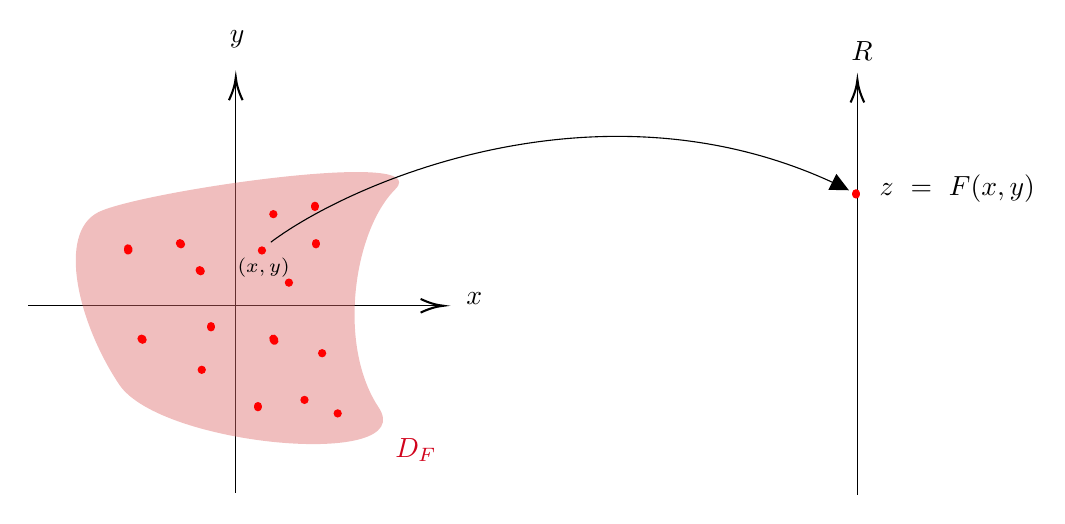
\begin{tikzpicture}[x=0.75pt,y=0.75pt,yscale=-1,xscale=1]
        %uncomment if require: \path (0,300); %set diagram left start at 0, and has height of 300
        %Straight Lines [id:da2454744672554513] 
        \draw    (30.4,163.6) -- (228.4,163.6) ;
        \draw [shift={(230.4,163.6)}, rotate = 180] [color={rgb, 255:red, 0; green, 0; blue, 0 }  ][line width=0.75]    (10.93,-3.29) .. controls (6.95,-1.4) and (3.31,-0.3) .. (0,0) .. controls (3.31,0.3) and (6.95,1.4) .. (10.93,3.29)   ;
        %Straight Lines [id:da9462448097326388] 
        \draw    (130.4,253.6) -- (130.4,55.6) ;
        \draw [shift={(130.4,53.6)}, rotate = 90] [color={rgb, 255:red, 0; green, 0; blue, 0 }  ][line width=0.75]    (10.93,-3.29) .. controls (6.95,-1.4) and (3.31,-0.3) .. (0,0) .. controls (3.31,0.3) and (6.95,1.4) .. (10.93,3.29)   ;
        %Shape: Polygon Curved [id:ds3375181141487479] 
        \draw  [draw opacity=0][fill={rgb, 255:red, 221; green, 107; blue, 107 }  ,fill opacity=0.44 ] (64.2,118.5) .. controls (84.2,108.5) and (227.2,87.5) .. (207.2,107.5) .. controls (187.2,127.5) and (179.2,182.5) .. (199.2,212.5) .. controls (219.2,242.5) and (94.2,231.5) .. (74.2,201.5) .. controls (54.2,171.5) and (44.2,128.5) .. (64.2,118.5) -- cycle ;
        %Shape: Free Drawing [id:dp9204827379504648] 
        \draw  [color={rgb, 255:red, 255; green, 0; blue, 0 }  ,draw opacity=1 ][line width=3] [line join = round][line cap = round] (78.5,135.95) .. controls (78.5,136.28) and (78.83,136.95) .. (78.5,136.95) ;
        %Shape: Free Drawing [id:dp7849387766178008] 
        \draw  [color={rgb, 255:red, 255; green, 0; blue, 0 }  ,draw opacity=1 ][line width=3] [line join = round][line cap = round] (85,179.45) .. controls (85,179.69) and (85.26,179.95) .. (85.5,179.95) ;
        %Shape: Free Drawing [id:dp46987595803015936] 
        \draw  [color={rgb, 255:red, 255; green, 0; blue, 0 }  ,draw opacity=1 ][line width=3] [line join = round][line cap = round] (103.5,133.45) .. controls (103.74,133.45) and (104,133.71) .. (104,133.95) ;
        %Shape: Free Drawing [id:dp7703404610517858] 
        \draw  [color={rgb, 255:red, 255; green, 0; blue, 0 }  ,draw opacity=1 ][line width=3] [line join = round][line cap = round] (148.5,179.45) .. controls (148.67,179.78) and (148.83,180.12) .. (149,180.45) ;
        %Shape: Free Drawing [id:dp19881301407247098] 
        \draw  [color={rgb, 255:red, 255; green, 0; blue, 0 }  ,draw opacity=1 ][line width=3] [line join = round][line cap = round] (148.5,119.45) .. controls (148.5,119.45) and (148.5,119.45) .. (148.5,119.45) ;
        %Shape: Free Drawing [id:dp5710424755546443] 
        \draw  [color={rgb, 255:red, 255; green, 0; blue, 0 }  ,draw opacity=1 ][line width=3] [line join = round][line cap = round] (168.5,115.45) .. controls (168.5,115.62) and (168.5,115.78) .. (168.5,115.95) ;
        %Shape: Free Drawing [id:dp5794203159577371] 
        \draw  [color={rgb, 255:red, 255; green, 0; blue, 0 }  ,draw opacity=1 ][line width=3] [line join = round][line cap = round] (156,152.45) .. controls (156,152.45) and (156,152.45) .. (156,152.45) ;
        %Shape: Free Drawing [id:dp48323620450280513] 
        \draw  [color={rgb, 255:red, 255; green, 0; blue, 0 }  ,draw opacity=1 ][line width=3] [line join = round][line cap = round] (114,194.45) .. controls (114,194.45) and (114,194.45) .. (114,194.45) ;
        %Shape: Free Drawing [id:dp5146781872742409] 
        \draw  [color={rgb, 255:red, 255; green, 0; blue, 0 }  ,draw opacity=1 ][line width=3] [line join = round][line cap = round] (163.5,208.95) .. controls (163.5,208.95) and (163.5,208.95) .. (163.5,208.95) ;
        %Shape: Free Drawing [id:dp5139020858297133] 
        \draw  [color={rgb, 255:red, 255; green, 0; blue, 0 }  ,draw opacity=1 ][line width=3] [line join = round][line cap = round] (169,133.45) .. controls (169,133.62) and (169,133.78) .. (169,133.95) ;
        %Shape: Free Drawing [id:dp19700765387729546] 
        \draw  [color={rgb, 255:red, 255; green, 0; blue, 0 }  ,draw opacity=1 ][line width=3] [line join = round][line cap = round] (113,146.45) .. controls (113.24,146.45) and (113.5,146.71) .. (113.5,146.95) ;
        %Shape: Free Drawing [id:dp834751610315057] 
        \draw  [color={rgb, 255:red, 255; green, 0; blue, 0 }  ,draw opacity=1 ][line width=3] [line join = round][line cap = round] (118.5,173.45) .. controls (118.5,173.62) and (118.5,173.78) .. (118.5,173.95) ;
        %Shape: Free Drawing [id:dp726934650472843] 
        \draw  [color={rgb, 255:red, 255; green, 0; blue, 0 }  ,draw opacity=1 ][line width=3] [line join = round][line cap = round] (143,136.95) .. controls (143,136.95) and (143,136.95) .. (143,136.95) ;
        %Shape: Free Drawing [id:dp8110315242879534] 
        \draw  [color={rgb, 255:red, 255; green, 0; blue, 0 }  ,draw opacity=1 ][line width=3] [line join = round][line cap = round] (172,186.45) .. controls (172,186.45) and (172,186.45) .. (172,186.45) ;
        %Shape: Free Drawing [id:dp9233705674999151] 
        \draw  [color={rgb, 255:red, 255; green, 0; blue, 0 }  ,draw opacity=1 ][line width=3] [line join = round][line cap = round] (179.5,215.45) .. controls (179.5,215.45) and (179.5,215.45) .. (179.5,215.45) ;
        %Shape: Free Drawing [id:dp5938234305401566] 
        \draw  [color={rgb, 255:red, 255; green, 0; blue, 0 }  ,draw opacity=1 ][line width=3] [line join = round][line cap = round] (141,211.95) .. controls (141,212.12) and (141,212.28) .. (141,212.45) ;
        %Straight Lines [id:da8978492632675772] 
        \draw    (429.9,254.7) -- (429.9,56.7) ;
        \draw [shift={(429.9,54.7)}, rotate = 90] [color={rgb, 255:red, 0; green, 0; blue, 0 }  ][line width=0.75]    (10.93,-3.29) .. controls (6.95,-1.4) and (3.31,-0.3) .. (0,0) .. controls (3.31,0.3) and (6.95,1.4) .. (10.93,3.29)   ;
        %Shape: Free Drawing [id:dp07629673461708475] 
        \draw  [color={rgb, 255:red, 255; green, 0; blue, 0 }  ,draw opacity=1 ][line width=3] [line join = round][line cap = round] (429.3,109.45) .. controls (429.3,109.62) and (429.3,109.78) .. (429.3,109.95) ;
        %Curve Lines [id:da02270658119899094] 
        \draw    (147.3,132.95) .. controls (187.1,103.1) and (310.06,50.48) .. (424.08,107.09) ;
        \draw [shift={(425.8,107.95)}, rotate = 206.86] [fill={rgb, 255:red, 0; green, 0; blue, 0 }  ][line width=0.08]  [draw opacity=0] (8.93,-4.29) -- (0,0) -- (8.93,4.29) -- cycle;

        % Text Node
        \draw (240.24,155.88) node [anchor=north west][inner sep=0.75pt]    {$x$};
        % Text Node
        \draw (126.24,29.88) node [anchor=north west][inner sep=0.75pt]    {$y$};
        % Text Node
        \draw (206,226.4) node [anchor=north west][inner sep=0.75pt]    {$\textcolor[rgb]{0.82,0.01,0.11}{D_{F}}$};
        % Text Node
        \draw (129.96,139.49) node [anchor=north west][inner sep=0.75pt]  [font=\scriptsize,rotate=-359.72]  {$( x,y)$};
        % Text Node
        \draw (425.74,34.88) node [anchor=north west][inner sep=0.75pt]    {$\mathbb{R}$};
        % Text Node
        \draw (439.3,99.4) node [anchor=north west][inner sep=0.75pt]    {$z\ =\ F( x,y)$};
        \end{tikzpicture}
    \caption{Funçaõ de duas variáveis reais}
    \label{fig:variasvariaveis}
\end{figure}

\begin{remark}
    Quando não especificamos o domínio da função, fica subentendido que se trata do ``maior'' subconjunto de \(\R^2\) para o qual a função faz sentido.
\end{remark}

\begin{example}
    Seja \(f(x,y) = \frac{x+y}{x-y}\). Vamos determinar o domínio e a imagem de \(f\).

    Note que devemos ter \[x-y \neq 0 \Rightarrow x\neq y.\] Logo \(D_f = \{(x,y)\in\R^2 : x\neq y\}\).
    \begin{figure}[htbp]
        \centering 
            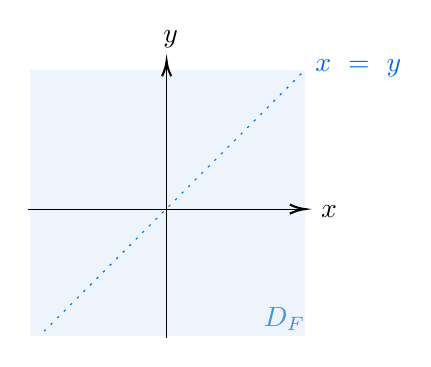
\begin{tikzpicture}[x=0.5pt,y=0.5pt,yscale=-1,xscale=1]
                %Shape: Rectangle [id:dp9118034779997847] 
                \draw  [draw opacity=0][fill={rgb, 255:red, 74; green, 144; blue, 226 }  ,fill opacity=0.1 ] (51.35,80.33) -- (250.15,80.33) -- (250.15,272.09) -- (51.35,272.09) -- cycle ;
                %Straight Lines [id:da2642326786185505] 
                \draw    (50.4,180.6) -- (248.4,180.6) ;
                \draw [shift={(250.4,180.6)}, rotate = 180] [color={rgb, 255:red, 0; green, 0; blue, 0 }  ][line width=0.75]    (10.93,-3.29) .. controls (6.95,-1.4) and (3.31,-0.3) .. (0,0) .. controls (3.31,0.3) and (6.95,1.4) .. (10.93,3.29)   ;
                %Straight Lines [id:da8917343736599169] 
                \draw    (150.4,273.6) -- (150.4,75.6) ;
                \draw [shift={(150.4,73.6)}, rotate = 90] [color={rgb, 255:red, 0; green, 0; blue, 0 }  ][line width=0.75]    (10.93,-3.29) .. controls (6.95,-1.4) and (3.31,-0.3) .. (0,0) .. controls (3.31,0.3) and (6.95,1.4) .. (10.93,3.29)   ;
                %Straight Lines [id:da21790853074689742] 
                \draw [color={rgb, 255:red, 0; green, 105; blue, 228 }  ,draw opacity=1 ] [dash pattern={on 0.84pt off 2.51pt}]  (61.9,268.83) -- (250.15,80.33) ;

                % Text Node
                \draw (260.24,175.88) node [anchor=north west][inner sep=0.75pt]    {$x$};
                % Text Node
                \draw (146.24,49.88) node [anchor=north west][inner sep=0.75pt]    {$y$};
                % Text Node
                \draw (256,70.32) node [anchor=north west][inner sep=0.75pt]  [color={rgb, 255:red, 74; green, 144; blue, 226 }  ,opacity=1 ]  {$\textcolor[rgb]{0,0.41,0.89}{x\ =\ y}$};
                % Text Node
                \draw (218.8,249.52) node [anchor=north west][inner sep=0.75pt]  [color={rgb, 255:red, 74; green, 144; blue, 226 }  ,opacity=1 ]  {$D_{F}$};
                \end{tikzpicture}
        \caption{Domínio de \(f(x,y) = \frac{x+y}{x-y}\)}
        \label{fig:pol1}
    \end{figure}

    Além disso, \[\operatorname{Im}_f = \left\{z = \frac{x+y}{x-y} : x\neq y\right\} \overbrace{=}^{\text{ (parece) }} \R.\]
\end{example}

\begin{example}
    Seja \(f(x,y) = \sqrt{y-x} + \sqrt{1-y}\). Para determinar o domínio de \(f\) devemos ter
        \begin{enumerate}
            \item[i)] \(y-x \geq 0\), portanto \(y\geq x\);
            \item[ii)] \(1-y \geq 0\), daí \(y\leq 1\).
        \end{enumerate}
    Logo \[D_f = \left\{(x,y)\in\R^2 : y\leq 1 \text{ e } y\geq x\right\}.\]
        \begin{figure}[htbp]
            \centering
                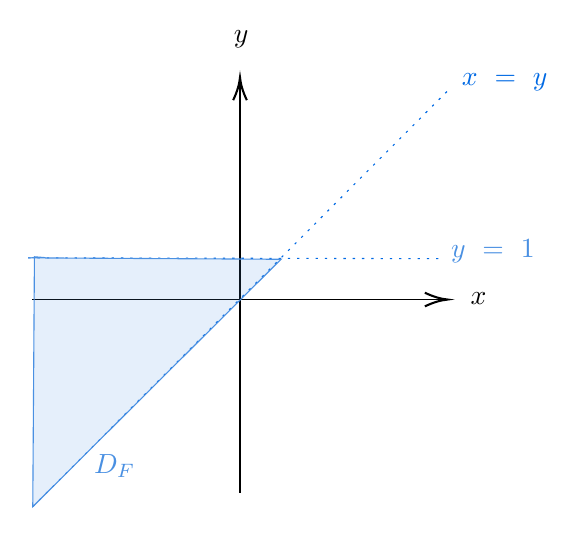
\begin{tikzpicture}[x=0.75pt,y=0.75pt,yscale=-1,xscale=1]
                    %uncomment if require: \path (0,300); %set diagram left start at 0, and has height of 300
                    %Straight Lines [id:da2642326786185505] 
                    \draw    (50.4,180.6) -- (248.4,180.6) ;
                    \draw [shift={(250.4,180.6)}, rotate = 180] [color={rgb, 255:red, 0; green, 0; blue, 0 }  ][line width=0.75]    (10.93,-3.29) .. controls (6.95,-1.4) and (3.31,-0.3) .. (0,0) .. controls (3.31,0.3) and (6.95,1.4) .. (10.93,3.29)   ;
                    %Straight Lines [id:da8917343736599169] 
                    \draw    (150.4,273.6) -- (150.4,75.6) ;
                    \draw [shift={(150.4,73.6)}, rotate = 90] [color={rgb, 255:red, 0; green, 0; blue, 0 }  ][line width=0.75]    (10.93,-3.29) .. controls (6.95,-1.4) and (3.31,-0.3) .. (0,0) .. controls (3.31,0.3) and (6.95,1.4) .. (10.93,3.29)   ;
                    %Straight Lines [id:da21790853074689742] 
                    \draw [color={rgb, 255:red, 0; green, 105; blue, 228 }  ,draw opacity=1 ] [dash pattern={on 0.84pt off 2.51pt}]  (50.56,280.4) -- (250.15,80.33) ;
                    %Straight Lines [id:da7680119420914071] 
                    \draw [color={rgb, 255:red, 0; green, 105; blue, 228 }  ,draw opacity=1 ] [dash pattern={on 0.84pt off 2.51pt}]  (48.37,160.51) -- (248.77,160.91) ;
                    %Shape: Polygon [id:ds21875134066080693] 
                    \draw  [color={rgb, 255:red, 74; green, 144; blue, 226 }  ,draw opacity=1 ][fill={rgb, 255:red, 74; green, 144; blue, 226 }  ,fill opacity=0.14 ] (48.37,160.51) -- (170.16,161.2) -- (50.56,280.4) -- (51.36,160) -- (56.56,160.4) -- cycle ;

                    % Text Node
                    \draw (260.24,175.88) node [anchor=north west][inner sep=0.75pt]    {$x$};
                    % Text Node
                    \draw (146.24,49.88) node [anchor=north west][inner sep=0.75pt]    {$y$};
                    % Text Node
                    \draw (256,70.32) node [anchor=north west][inner sep=0.75pt]  [color={rgb, 255:red, 74; green, 144; blue, 226 }  ,opacity=1 ]  {$\textcolor[rgb]{0,0.41,0.89}{x\ =\ y}$};
                    % Text Node
                    \draw (78.8,253.92) node [anchor=north west][inner sep=0.75pt]  [color={rgb, 255:red, 74; green, 144; blue, 226 }  ,opacity=1 ]  {$D_{F}$};
                    % Text Node
                    \draw (250.8,150.72) node [anchor=north west][inner sep=0.75pt]  [color={rgb, 255:red, 74; green, 144; blue, 226 }  ,opacity=1 ]  {$y\ =\ 1$};
                \end{tikzpicture}                    
            \caption{Domínio de \(f(x,y) = \sqrt{y-x} + \sqrt{1-y}\)}
            \label{fig:raiz1}
        \end{figure}

        Além disso, \[\operatorname{Im}_f = \left\{ z = \sqrt{y-x} + \sqrt{1-y} : y\leq 1 \text{ e } y\geq x \right\} = \{z \geq 0\} = [0\infty).\]
\end{example}

\begin{example}
    Seja \(f(x,y) = x^2 - y^2\). Aqui não temos nenhuma restrição ao domínio, portanto \(D_f = \R^2\). Além disso, \[\operatorname{Im}_f = \left\{ z = x^2 - y^2 : (x,y)\in\R^2 \right\} = \R.\]
\end{example}

\begin{example}
    Consideramos \(f(x,y) = \sqrt{9 - x^2 - y^2}\). Então devemos ter \[9 - x^2 - y^2 \geq 0 \Rightarrow x^2 + y^2 \leq 9.\] Logo \[D_f = \left\{ (x,y)\in\R^2 : x^2 + y^2 \leq 9 \right\}\]
    \begin{figure}[htbp]
        \centering
            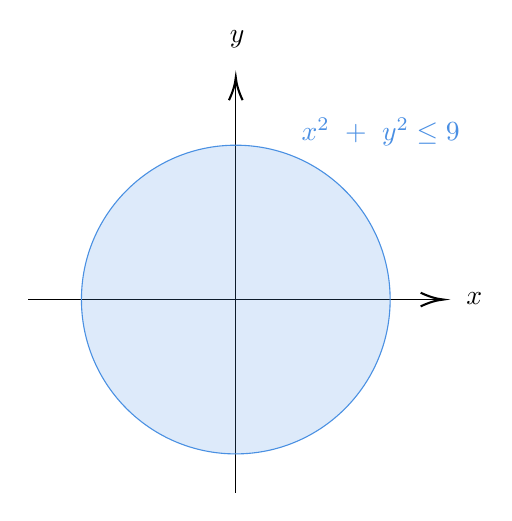
\begin{tikzpicture}[x=0.75pt,y=0.75pt,yscale=-1,xscale=1]
                %Straight Lines [id:da2642326786185505] 
                \draw    (50.4,180.6) -- (248.4,180.6) ;
                \draw [shift={(250.4,180.6)}, rotate = 180] [color={rgb, 255:red, 0; green, 0; blue, 0 }  ][line width=0.75]    (10.93,-3.29) .. controls (6.95,-1.4) and (3.31,-0.3) .. (0,0) .. controls (3.31,0.3) and (6.95,1.4) .. (10.93,3.29)   ;
                %Straight Lines [id:da8917343736599169] 
                \draw    (150.4,273.6) -- (150.4,75.6) ;
                \draw [shift={(150.4,73.6)}, rotate = 90] [color={rgb, 255:red, 0; green, 0; blue, 0 }  ][line width=0.75]    (10.93,-3.29) .. controls (6.95,-1.4) and (3.31,-0.3) .. (0,0) .. controls (3.31,0.3) and (6.95,1.4) .. (10.93,3.29)   ;
                %Shape: Circle [id:dp15347112833091703] 
                \draw  [color={rgb, 255:red, 74; green, 144; blue, 226 }  ,draw opacity=1 ][fill={rgb, 255:red, 74; green, 144; blue, 226 }  ,fill opacity=0.19 ] (76.03,180.6) .. controls (76.03,139.53) and (109.33,106.23) .. (150.4,106.23) .. controls (191.47,106.23) and (224.77,139.53) .. (224.77,180.6) .. controls (224.77,221.67) and (191.47,254.97) .. (150.4,254.97) .. controls (109.33,254.97) and (76.03,221.67) .. (76.03,180.6) -- cycle ;

                % Text Node
                \draw (260.24,175.88) node [anchor=north west][inner sep=0.75pt]    {$x$};
                % Text Node
                \draw (146.24,49.88) node [anchor=north west][inner sep=0.75pt]    {$y$};
                % Text Node
                \draw (180.8,91.64) node [anchor=north west][inner sep=0.75pt]    {$\textcolor[rgb]{0.29,0.56,0.89}{x^{2} \ +\ y^{2} \leq 9}$};
            \end{tikzpicture}                    
        \caption{Domínio de \(f(x,y) = \sqrt{9 - x^2 - y^2}\)}
        \label{fig:raiz2}
    \end{figure}
    Além disso \[\operatorname{Im}_f = \left\{ z = \sqrt{9 - x^2 - y^2} : x^2 + y^2 \leq 9 \right\},\] agora, notando que
        \begin{align*}
            0 \leq x^2 + y^2 \leq 9
                & \Leftrightarrow -9 \leq -x^2 - y^2 \leq 0 \\
                & \Leftrightarrow 0 \leq 9 - x^2 - y^2 \leq 9 \\
                & \Leftrightarrow 0 \leq \sqrt{9 - x^2 - y^2} \leq 3,
        \end{align*}
    temos que \(\operatorname{Im}_f = [0,3]\).
\end{example}

\begin{example}
    Seja \(f(x,y) = \frac{1}{\sqrt{4 - x^2 - y^2}}\).

    Devemos ter \[4 - x^2 - y^2 > 0 \Rightarrow x^2 + y^2 \leq 4.\] Logo \[D_f = \left\{(x,y)\in\R^2 : x^2 + y^2 < 4 \right\}.\]
        \begin{figure}[htbp]
            \centering
                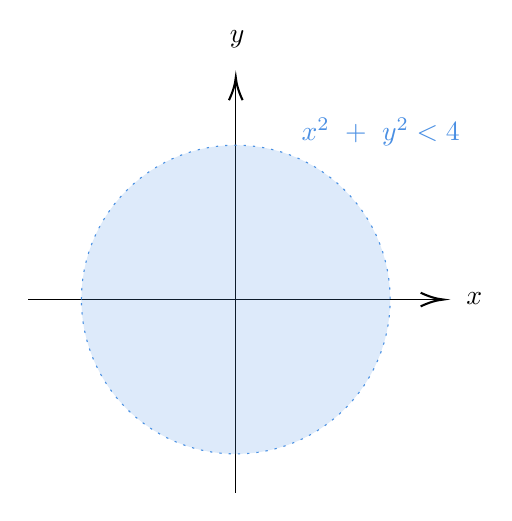
\begin{tikzpicture}[x=0.75pt,y=0.75pt,yscale=-1,xscale=1]
                    %Straight Lines [id:da2642326786185505] 
                    \draw    (50.4,180.6) -- (248.4,180.6) ;
                    \draw [shift={(250.4,180.6)}, rotate = 180] [color={rgb, 255:red, 0; green, 0; blue, 0 }  ][line width=0.75]    (10.93,-3.29) .. controls (6.95,-1.4) and (3.31,-0.3) .. (0,0) .. controls (3.31,0.3) and (6.95,1.4) .. (10.93,3.29)   ;
                    %Straight Lines [id:da8917343736599169] 
                    \draw    (150.4,273.6) -- (150.4,75.6) ;
                    \draw [shift={(150.4,73.6)}, rotate = 90] [color={rgb, 255:red, 0; green, 0; blue, 0 }  ][line width=0.75]    (10.93,-3.29) .. controls (6.95,-1.4) and (3.31,-0.3) .. (0,0) .. controls (3.31,0.3) and (6.95,1.4) .. (10.93,3.29)   ;
                    %Shape: Circle [id:dp15347112833091703] 
                    \draw  [color={rgb, 255:red, 74; green, 144; blue, 226 }  ,draw opacity=1 ][fill={rgb, 255:red, 74; green, 144; blue, 226 }  ,fill opacity=0.19 ][dash pattern={on 0.84pt off 2.51pt}] (76.03,180.6) .. controls (76.03,139.53) and (109.33,106.23) .. (150.4,106.23) .. controls (191.47,106.23) and (224.77,139.53) .. (224.77,180.6) .. controls (224.77,221.67) and (191.47,254.97) .. (150.4,254.97) .. controls (109.33,254.97) and (76.03,221.67) .. (76.03,180.6) -- cycle ;

                    % Text Node
                    \draw (260.24,175.88) node [anchor=north west][inner sep=0.75pt]    {$x$};
                    % Text Node
                    \draw (146.24,49.88) node [anchor=north west][inner sep=0.75pt]    {$y$};
                    % Text Node
                    \draw (180.8,91.64) node [anchor=north west][inner sep=0.75pt]    {$\textcolor[rgb]{0.29,0.56,0.89}{x^{2} \ +\ y^{2} < 4}$};
                \end{tikzpicture}                    
            \caption{Domínio de \(f(x,y) = \frac{1}{\sqrt{4 - x^2 - y^2}}\)}
            \label{fig:raiz3}
        \end{figure}

    Além disso, \[\operatorname{Im}_f = \left\{ z = \frac{1}{\sqrt{4 - x^2 - y^2}} : x^2 + y^2 < 4 \right\},\] mas notando que
        \begin{align*}
            0 \leq x^2 + y^2 < 4
                & \Leftrightarrow  - 4 \leq -x^2 - y^2 \leq 0 \\
                & \Leftrightarrow 0 < 4 - x^2 - y^2 \leq 4 \\
                & \Leftrightarrow 0 < \sqrt{4 - x^2 - y^2} \leq 2 \\
                & \Leftrightarrow \frac{1}{\sqrt{4 - x^2 - y^2}} \geq \frac{1}{2},
        \end{align*}
    concluímos que \[\operatorname{Im}_f = \left\{z \geq \frac{1}{2}\right\} = \left[\frac{1}{2},\infty\right).\]
\end{example}

\begin{exercise}
    Estude \(D_f\) e \(\operatorname{Im}_f\) para cada função \(f\) abaixo.
        \begin{enumerate}
            \item \(f(x,y) = \frac{\sqrt{x+y+1}}{x-1}\).
            \item \(f(x,y) = \sin(xy)\).
            \item \(f(x,y) = \frac{1}{xy}\).
            \item \(f(x,y) = 5x^2 - 3x\).
        \end{enumerate}
\end{exercise}

A seguir temos algumas definições que também são exemplos de funções de duas variáveis reais a valores reais.

\begin{definition}
    Uma \textbf{função polinomial}\index{Funções de duas variáveis a valores reais! Polinomial} de duas variáveis reais a valores reais é uma função \(f:\R^2 \to \R\) dada por \[f(x,y) = \sum_{m+n\leq p} a_{m,n}x^m y^n,\] no qual \(p\in\N\) é fixo (chamado \textbf{grau do polinômio}) e \(a_{m,n}\in\R\) são dados.
\end{definition}

\begin{example}
    \begin{enumerate}
        \item \(f(x,y) = 3x^3 y^2 - \frac{1}{3} x y + \sqrt{2}\) é uma função polinomial de grau 5.
        \item \(f(x,y) = ax + by + c\), com \(a,b,c\in\R\) é uma função polinomial de grau 1. Chamamos tal função de \textbf{função afim}\index{Funções de duas variáveis a valores reais! Afim}.
        \item \(f(x,y) = ax + by\), com \(a,b\in\R\) é uma função polinomial (mais ainda, é uma função afim) e tal função é chamada \textbf{função linear}\index{Funções de duas variáveis a valores reais! Linear}.
    \end{enumerate}
\end{example}

\begin{definition}
    Toda função \(f:D_f \subset\R^2 \to \R\) dada por \[f(x,y) = \frac{p(x,y)}{q(x,y)},\] com \(p\) e \(q\) funções polinomiais, é chamada \textbf{função racional}\index{Funções de duas variáveis a valores reais! Racional} e \[\{D_f = (x,y)\in\R^2 : q(x,y)\neq 0\}.\]
\end{definition}

\begin{example}
    \begin{enumerate}
        \item \(f(x,y) = \frac{x+y}{x-y}\) é uma função racional e \(D_f = \{(x,y)\in\R^2 : x\neq y\}\).
        \item \(g(x,y) = \frac{x^2 - 3xy + 1}{x^2 y^2 + 1}\) é uma função racinal e \(D_g = \R^2\).
    \end{enumerate}
\end{example}

\begin{definition}
    Uma função \(f:D_f \subset \R^2 \to \R\) se chama \textbf{função homogênea}\index{Funções de duas variáveis a valores reais! Homogêneas} de grau \(\lambda\) se \[f(tx,ty) = t^\lambda f(x,y)\] para todo \(t>0\) e todo \((x,y)\in D_f\) tais que \((tx,ty)\in D_f\).
\end{definition}

\begin{example}
    \begin{enumerate}
        \item \(f(x,y) = 3x^2 + 5xy + y^2\) é homogênea de grau \(2\).
        
        De fato, temos que \(D_f = \R^2\). Portanto, para todo \(t>0\) e \((x,y)\in D_f\) temos \((tx,ty)\in D_f\) e
            \begin{align*}
                f(tx,ty)
                    & = 3(tx)^2 + 5(tx)(ty) + (ty)^2 \\
                    & = 3t^2x^2 + 5t^2xy + t^2y^2 \\
                    & = t^2(3x^2+5xy+y^2) \\
                    & = t^2 f(x,y)
            \end{align*}
        portanto \(f\) é homogênea de grau \(2\).
        \item \(f(x,y) = \frac{xe^{\frac{x}{y}}}{x^2 + y^2}\) é homogênea de grau \(-1\). De fato, \(D_f = \{(x,y)\in\R^2 : y\neq 0\}\) e, para todo \(t>0\) e \((x,y)\in D_f\), temos \((tx,ty)\in D_f\). Além disso,
            \begin{align*}
                f(tx,ty)
                    & = \frac{(tx)e^{\frac{(tx)}{(ty)}}}{(tx)^2 + (ty)^2} \\
                    & = t \frac{xe^{\frac{x}{y}}}{t^2x^2 + t^2y^2} \\
                    & = \frac{xe^{\frac{x}{y}}}{t(x^2 + y^2)} = \frac{1}{t} \frac{xe^{\frac{x}{y}}}{x^2 + y^2} = t^{-1} f(x,y).
            \end{align*}
    \end{enumerate}
\end{example}

\begin{exercise}
    Determine se \(f(x,y) = 2x + y + 5\) é homogênea.
\end{exercise}

\section{Gráficos e Curvas de nível}

Lembre que o gráfico de uma função \(f:I\subset\R \to \R\) é uma curva \(C\) com equação \(y = f(x)\), ou seja \[C = \{(x,y)\in\R^2 : y = f(x), x\in I\}.\]
        % \begin{figure}[htbp]
        %     \centering
        %         \begin{tikzpicture}[x=1pt,y=1pt,yscale=-1,xscale=1]
        %             %Straight Lines [id:da2642326786185505] 
        %             \draw    (50.4,180.6) -- (248.4,180.6) ;
        %             \draw [shift={(250.4,180.6)}, rotate = 180] [color={rgb, 255:red, 0; green, 0; blue, 0 }  ][line width=0.75]    (10.93,-3.29) .. controls (6.95,-1.4) and (3.31,-0.3) .. (0,0) .. controls (3.31,0.3) and (6.95,1.4) .. (10.93,3.29)   ;
        %             %Straight Lines [id:da8917343736599169] 
        %             \draw    (150.4,273.6) -- (150.4,75.6) ;
        %             \draw [shift={(150.4,73.6)}, rotate = 90] [color={rgb, 255:red, 0; green, 0; blue, 0 }  ][line width=0.75]    (10.93,-3.29) .. controls (6.95,-1.4) and (3.31,-0.3) .. (0,0) .. controls (3.31,0.3) and (6.95,1.4) .. (10.93,3.29)   ;
        %             %Curve Lines [id:da6261892147437338] 
        %             \draw [color={rgb, 255:red, 74; green, 144; blue, 226 }  ,draw opacity=1 ]   (66.16,147.2) .. controls (82.16,92) and (206.96,162.4) .. (232.16,121.2) ;
        %             %Shape: Free Drawing [id:dp09709473855176909] 
        %             \draw  [color={rgb, 255:red, 74; green, 144; blue, 226 }  ,draw opacity=1 ][line width=3] [line join = round][line cap = round] (130.72,126.8) .. controls (130.72,126.8) and (130.72,126.8) .. (130.72,126.8) ;
        %             %Straight Lines [id:da7274654232721021] 
        %             \draw    (129.92,176) -- (129.92,184.8) ;
        %             %Straight Lines [id:da22804172354165553] 
        %             \draw    (148.63,127.65) -- (153.13,127.82) ;

        %             % Text Node
        %             \draw (260.24,175.88) node [anchor=north west][inner sep=0.75pt]    {$x$};
        %             % Text Node
        %             \draw (146.24,49.88) node [anchor=north west][inner sep=0.75pt]    {$y$};
        %             % Text Node
        %             \draw (227.12,69.04) node [anchor=north west][inner sep=0.75pt]    {$\mathbb{R}^{2}$};
        %             % Text Node
        %             \draw (236.72,103.24) node [anchor=north west][inner sep=0.75pt]    {$\textcolor[rgb]{0.29,0.56,0.89}{C}$};
        %             % Text Node
        %             \draw (122.32,115.24) node [anchor=north west][inner sep=0.75pt]  [font=\normalsize]  {$\textcolor[rgb]{0.29,0.56,0.89}{( x,y)}$};
        %             % Text Node
        %             \draw (124.32,182.44) node [anchor=north west][inner sep=0.75pt]  [font=\normalsize]  {$x$};
        %             % Text Node
        %             \draw (155.6,117.2) node [anchor=north west][inner sep=0.75pt]  [font=\normalsize]  {$y$};
        %         \end{tikzpicture}                    
        %     \caption{Gráfico de uma função real}
        %     \label{fig:grafico1}
        % \end{figure}

Qual seria o gráfico de uma função de duas variáveis \(f: D_f \subset\R^2 \to \R\)?

\begin{definition}
    Seja \(f:D_f\subset\R^2 \to \R\) uma função de duas variáveis reais a valores reais. O conjunto \[G_f = \{(x,y,z)\in\R^3 : z = f(x,y),\, (x,y)\in D_f\}\] é chamado \textbf{gráfico} de \(f\)\index{Funções de duas variáveis a valores reais! Gráfico}.
\end{definition}

Em outras palavras, o gráfico de uma função de duas variáveis reais é uma superfície \(
S\) com equação \(z = f(x,y)\).
        \begin{figure}[htbp]
            \centering
                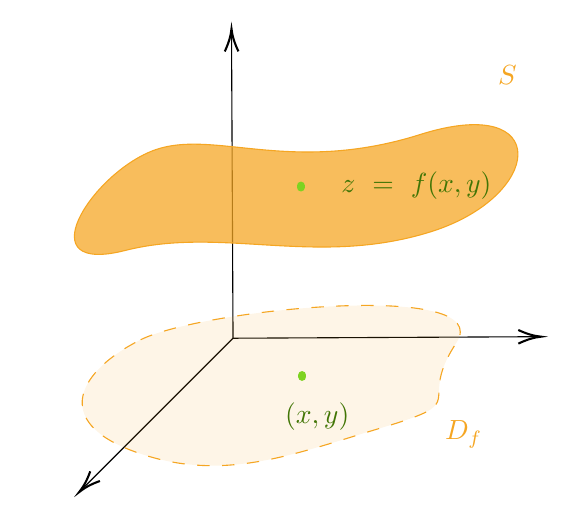
\begin{tikzpicture}[x=0.75pt,y=0.75pt,yscale=-1,xscale=1]
                    %Straight Lines [id:da2642326786185505] 
                    %Straight Lines [id:da8554379595110243] 
                    \draw    (290.62,182.37) -- (289.89,35.25) ;
                    \draw [shift={(289.88,33.25)}, rotate = 89.71] [color={rgb, 255:red, 0; green, 0; blue, 0 }  ][line width=0.75]    (10.93,-3.29) .. controls (6.95,-1.4) and (3.31,-0.3) .. (0,0) .. controls (3.31,0.3) and (6.95,1.4) .. (10.93,3.29)   ;
                    %Straight Lines [id:da319707950834352] 
                    \draw    (290.62,182.37) -- (437,181.64) ;
                    \draw [shift={(439,181.63)}, rotate = 179.71] [color={rgb, 255:red, 0; green, 0; blue, 0 }  ][line width=0.75]    (10.93,-3.29) .. controls (6.95,-1.4) and (3.31,-0.3) .. (0,0) .. controls (3.31,0.3) and (6.95,1.4) .. (10.93,3.29)   ;
                    %Straight Lines [id:da5129903513774706] 
                    \draw    (290.62,182.37) -- (217.84,255.15) ;
                    \draw [shift={(216.43,256.56)}, rotate = 315] [color={rgb, 255:red, 0; green, 0; blue, 0 }  ][line width=0.75]    (10.93,-3.29) .. controls (6.95,-1.4) and (3.31,-0.3) .. (0,0) .. controls (3.31,0.3) and (6.95,1.4) .. (10.93,3.29)   ;
                    %Shape: Polygon Curved [id:ds9048558325300219] 
                    \draw  [color={rgb, 255:red, 245; green, 166; blue, 35 }  ,draw opacity=1 ][fill={rgb, 255:red, 245; green, 166; blue, 35 }  ,fill opacity=0.74 ] (250.56,92.6) .. controls (279.79,80.21) and (316.59,104.47) .. (380.83,84.22) .. controls (445.08,63.96) and (440.48,114.12) .. (385.58,131.18) .. controls (330.68,148.24) and (285.43,128.21) .. (238.69,140.08) .. controls (191.95,151.95) and (221.33,104.99) .. (250.56,92.6) -- cycle ;
                    %Shape: Polygon Curved [id:ds300471178509903] 
                    \draw  [color={rgb, 255:red, 245; green, 166; blue, 35 }  ,draw opacity=1 ][fill={rgb, 255:red, 245; green, 166; blue, 35 }  ,fill opacity=0.11 ][dash pattern={on 4.5pt off 4.5pt}] (246.11,183.11) .. controls (275.78,168.28) and (418.23,154.18) .. (398.2,184.6) .. controls (378.16,215.02) and (407.1,212.05) .. (362.58,225.4) .. controls (318.07,238.76) and (285.43,252.11) .. (243.88,237.27) .. controls (202.33,222.44) and (216.43,197.95) .. (246.11,183.11) -- cycle ;
                    %Shape: Free Drawing [id:dp6078280162757188] 
                    \draw  [color={rgb, 255:red, 126; green, 211; blue, 33 }  ,draw opacity=1 ][line width=3] [line join = round][line cap = round] (324.01,200.18) .. controls (324.01,200.43) and (324.01,200.67) .. (324.01,200.92) ;
                    %Shape: Free Drawing [id:dp8408010884228739] 
                    \draw  [color={rgb, 255:red, 126; green, 211; blue, 33 }  ,draw opacity=1 ][line width=3] [line join = round][line cap = round] (323.26,108.92) .. controls (323.26,109.17) and (323.26,109.42) .. (323.26,109.67) ;

                    % Text Node
                    \draw (417.12,49.91) node [anchor=north west][inner sep=0.75pt]  [color={rgb, 255:red, 245; green, 166; blue, 35 }  ,opacity=1 ]  {$S$};
                    % Text Node
                    \draw (391.59,221.03) node [anchor=north west][inner sep=0.75pt]  [color={rgb, 255:red, 245; green, 166; blue, 35 }  ,opacity=1 ]  {$D_{f}$};
                    % Text Node
                    \draw (314.45,212.19) node [anchor=north west][inner sep=0.75pt]  [font=\normalsize,color={rgb, 255:red, 65; green, 117; blue, 5 }  ,opacity=1 ]  {$( x,y)$};
                    % Text Node
                    \draw (341.53,100.91) node [anchor=north west][inner sep=0.75pt]  [font=\normalsize,color={rgb, 255:red, 65; green, 117; blue, 5 }  ,opacity=1 ]  {$z\ =\ f( x,y)$};
                \end{tikzpicture}                    
            \caption{Gráfico de uma função de várias variáveis reais}
            \label{fig:grafico2}
        \end{figure}
Note que \(S\) é uma superfície que está diretamente acima ou abaixo do seu domínio \(D_f\), o qual está no plano-xy.

\begin{example}[Plano]
    Esboce o \href{https://www.geogebra.org/m/mbrvtck9}{gráfico} da função \(f(x,y) = 3.\)
        \begin{figure}[htbp]
            \centering
            
\includegraphics[width = 0.4\textwidth]{Gráfico de f(x,y) = 3.png}               
            \caption{Gráfico de \(f(x,y) = 3\)}
            \label{fig:grafico3}
        \end{figure}
\end{example}

\begin{example}[Função linear]
    Esboce o \href{https://www.geogebra.org/classic/zvdw5ck4}{gráfico} da função afim \[f(x,y) = 6 - 3x - 2y.\]

    Temos que \(D_f = \R^2\) e \(\operatorname{Im}_f = \{z = 6 - 3x - 2y : (x,y)\in\R^2 \}\). 
    
    O gráfico de \(f\) é a superfície \(S\) de equação \(3x + 2y + z = 6\). No 1º octante,
        \begin{itemize}
            \item se \(x=0\), temos a reta \(2y + z = 6\) no plano yz,
            \item se \(y = 0\), temos a reta \(3x + z = 6\) no plano \(xz\), e
            \item se \(z = 0\), temos a reta \(3x + 2y = 6\) no plano \(xy\).
        \end{itemize}
        \begin{figure}[htbp]
            \centering
            
\includegraphics[width=0.7\textwidth]{Gráfico de f(x,y) = 6 - 3x - 2y.png}               
            \caption{Gráfico de \(f(x,y) = 6 -3x - 2y\)}
            \label{fig:grafico4}
        \end{figure}

    Formalmente, sabemos que a equação \(3x + 2y + z = 6\) representa o plano que passa pelo ponto \((0,0,6)\) e é normal ao vetor \(\eta = (3,2,1)\). Ou seja, \[(3,2,1)\cdot[(x,y,z)-(0,0,6)] = 0,\; \forall(x,y,z)\in P.\]
    
    \begin{remark}
    Em geral, o gráfico de uma função afim \(f(x,y) = ax + by + c\) é dado pela equação \[z = ax + by + x \text{ ou } ax + by - z = c\] que é o plano que passa pelo ponto \((0,0,c)\) e é normal ao vetor \(\eta = (a,b,-1)\).
\end{remark}
\end{example}

\begin{example}[Semiesfera]
    Esboce o \href{https://www.geogebra.org/m/jepwjjhe}{gráfico} de \(g(x,y) = \sqrt{9 - x^2 - y^2}\).

    Já vimos que \(D_g = \{(x,y)\in\R^2 : x^2 + y^2 \leq 9 \} \) e \(\operatorname{Im}_g = [0,3]\). Assim, o gráfico de \(g\) tem equação \[z = \sqrt{9 -x^2 - y^2}\] ou ainda \[z^2 = 9 - x^2 - y^2 \Leftrightarrow x^2 + y^2 + z^2 = 3^2.\]
    \begin{figure}[htbp]
        \centering
        
\includegraphics[width=0.75\textwidth]{Gráfico de f(x,y) = sqrt(9-x^2-y^2).png}               
        \caption{Gráfico de \(f(x,y) = \sqrt{9-x^2-y^2}\)}
        \label{fig:grafico5}
    \end{figure}

    Observe que o gráfico de \(g\) é só a metade superior da esfera uma vez que \(z\geq 0\).

    \textbf{Pergunta: } A esfera inteira pode ser representada por uma função de \(x\) e \(y\)?

    Lembre que uma esfera é o conjunto de todos os pontos que possuem a mesma distância de um certo ponto \(\mathcal{O}\). Se \(\mathcal{O} = (a,b,c)\), a equação da esfera de raio \(r\) e centro \(\mathcal{O}\) é o conjunto de todo \((x,y,z)\) tal que \[\|(x,y,z) - (a,b,c)\| = r,\] ou seja \[\sqrt{(x-a)^2 + (y-b)^2 + (z-c)^2} = r,\] ou ainda \[(x-a)^2 + (y-b)^2 + (z-c)^2 = r^2.\] Em particular, se \(\mathcal{O} = (0,0,0)\), então a equação fica \[x^2 + y^2 + z^2 = r^2.\]
\end{example}

\begin{example}[Parabolóide]
    Esboce o \href{https://www.geogebra.org/3d/zhbmek6q}{gráfico} de \(f(x,y) = x^2 + y^2\).

    Temos que \(D_f = \R^2\) e \[\operatorname{Im}_f = \{z = x^2 + y^2 : (x,y)\in\R^2\} = [0,\infty).\] O gráfico de \(f\) tem equação \(z = x^2 + y^2\).

    Para esboçar o gráfico de \(f\) notamos que
        \begin{itemize}
            \item se \(x = 0\), então \(z = y^2\), que é uma parábola no plano yz,
            \item se \(y=0\), temos uma parábola \(z = x^2\) no plano xz,
            \item em geral, se \(y = ax\), então \(z = x^2 + (ax)^2 = (1+a^2)x^2\), ou seja, temos uma parábola no plano (ax)z,
            \item se \(z = k\), temos \(x^2 + y^2 = k\), que é uma circunferência centrada na origem de raio \(\sqrt{k}\).
        \end{itemize}
    \begin{figure}[htbp]
        \centering
        
\includegraphics[width=0.7\textwidth]{Gráfico de f(x,y) = x^2 + y^2.png}               
        \caption{Gráfico de \(f(x,y) = x^2 + y^2\)}
        \label{fig:grafico6}
    \end{figure}
\end{example}

\begin{example}[Parabolóide elíptico]
    Esboce o \href{https://www.geogebra.org/3d/j49v7ctq}{gráfico} de \(h(x,y) = 4x^2 + y^2\).

    Temos que \(D_h = \R^2\) e \[\operatorname{Im}_h = \{z = 4x^2 + y^2 : (x,y)\in\R^2\} = [0,\infty].\] O gráfico de \(h\) tem equação \(z = 4x^2 + y^2\).

    Para esboçar o gráfico de \(f\) notamos que
        \begin{itemize}
            \item se \(x = 0\), então \(z = y^2\), que é uma parábola no plano yz,
            \item se \(y=0\), temos uma parábola \(z = 4x^2\) no plano xz,
            \item em geral, se \(y = ax\), então \(z = 4x^2 + (ax)^2 = (4+a^2)x^2\), ou seja, temos uma parábola no plano (ax)z,
            \item se \(z = k\), temos \(4x^2 + y^2 = k\), ou seja \[x^2 + \frac{y^2}{4} = \frac{k}{4} \Leftrightarrow \frac{x^2}{\frac{k}{4}} + \frac{y^2}{k} = 1,\] que são elipses no plano \(z=k\).
        \end{itemize}
    \begin{figure}[htbp]
        \centering
        
\includegraphics[width=0.7\textwidth]{Gráfico de f(x,y) = 4x^2 + y^2.png}
        \caption{Gráfico de \(f(x,y) = 4x^2 + y^2\)}
        \label{fig:grafico7}
    \end{figure}
\end{example}

Para exemplos de outras superfícies cilíndricas veja \cite[Seção 12.6]{stewart2}.

\begin{example}[Cone]
    Esboce o \href{https://www.geogebra.org/3d/jvjtjdam}{gráfico} da função \(f(x,y) = \sqrt{x^2 + y^2}\).

    Temos que \(D_f = \R^2\) e \(\operatorname{Im}_f = [0,\infty)\) (exercício).

    O gráfico de \(f\) tem equação \(z = \sqrt{x^2 + y^2}\), para esboça-lo notamos que
        \begin{itemize}
            \item se \(x=0\), então \(z = |y|\) no plano yz,
            \item se \(y=0\), temos \(z = |x|\) no plano xz,
            \item se \(z = k\), temos \(x^2 + y^2 = k\), que é uma circunferência no plano \(z=k\) centrada em \((0,0,k)\) e com raio \(\sqrt{k}\), e
            \item se \(y=ax\), então \(z = \sqrt{x^2 + a^2x^2} = |x|\sqrt{1+a^2}\) no plano (ax)z.
        \end{itemize}
    \begin{figure}[htbp]
        \centering
        
\includegraphics[width=0.6\textwidth]{Gráfico de f(x,y) = sqrt(x^2 + y^2).png}
        \caption{Gráfico de \(f(x,y) = \sqrt{x^2 + y^2}\)}
        \label{fig:grafico9}
    \end{figure}
\end{example}

A representação geométrica do gráfico de uma função de duas variáveis (muitas vezes) pode não ser fácil. Assim, quando queremos ter uma visão geométrica da função podemos usar um método que chamamos de \textbf{curvas de nível}.

\begin{definition}
    Sejam \(z = f(x,y)\) uma função de duas variáveis e \(k\in\operatorname{Im}_f\). O conjunto de todos os pontos \((x,y)\in D_f\) tais que \(f(x,y) = k\) é chamado \textbf{curva de nível}\index{Funções de duas variáveis a valores reais! Curva de nível} de \(f\) correspondente ao nível \(k\).
\end{definition}

% \begin{remark}[Curiosidade]
%     Essa técnica é empregada por cartógrafos nos mapas de contorno em que todos os pontos tem a mesma elevação.
% \end{remark}

Em outras palavras, uma curva de nível \(f(x,y) = k\) mostra, em \(D_f\), onde o gráfico de \(f\) tem altura \(k\).

Ou ainda, as curvas de nível \(f(x,y) = k\) são apenas traços do gráfico de \(f\) no plano horizontal \(z=k\) projetados no plano xy.

Assim, se traçarmos as curvas de nível de uma função e as vizualizamos elevadas para a superfície na altura indicada podemos ``imaginar'' o gráfico da função.
    \begin{figure}[htbp]
        \centering
            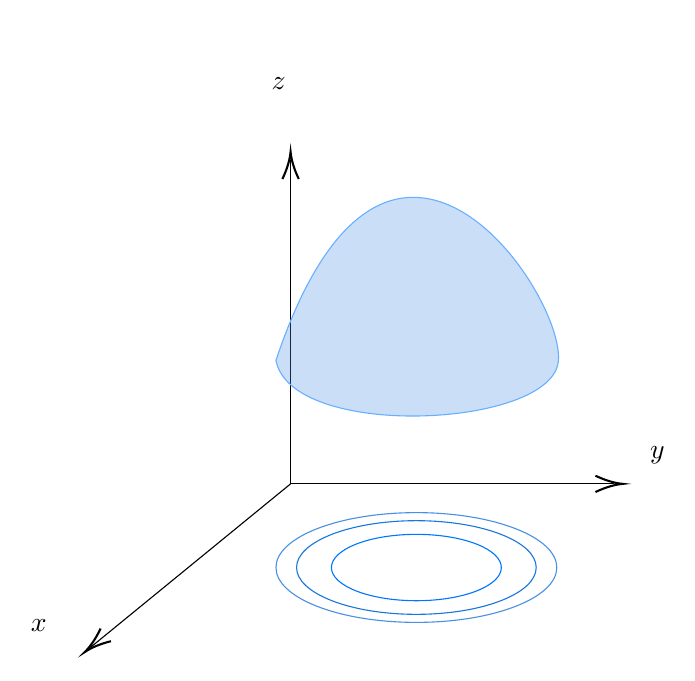
\begin{tikzpicture}[x=1.5pt,y=1.5pt,yscale=-1,xscale=1]
                %Straight Lines [id:da9147647358123466] 
                \draw    (81.2,210) -- (81.2,132) ;
                \draw [shift={(81.2,130)}, rotate = 90] [color={rgb, 255:red, 0; green, 0; blue, 0 }  ][line width=0.75]    (6.56,-1.97) .. controls (4.17,-0.84) and (1.99,-0.18) .. (0,0) .. controls (1.99,0.18) and (4.17,0.84) .. (6.56,1.97)   ;
                %Straight Lines [id:da20313754752615065] 
                \draw    (81.2,210) -- (159.2,210) ;
                \draw [shift={(161.2,210)}, rotate = 180] [color={rgb, 255:red, 0; green, 0; blue, 0 }  ][line width=0.75]    (6.56,-1.97) .. controls (4.17,-0.84) and (1.99,-0.18) .. (0,0) .. controls (1.99,0.18) and (4.17,0.84) .. (6.56,1.97)   ;
                %Straight Lines [id:da7849829970447654] 
                \draw    (81.2,210) -- (33.15,249.27) ;
                \draw [shift={(31.6,250.53)}, rotate = 320.74] [color={rgb, 255:red, 0; green, 0; blue, 0 }  ][line width=0.75]    (6.56,-1.97) .. controls (4.17,-0.84) and (1.99,-0.18) .. (0,0) .. controls (1.99,0.18) and (4.17,0.84) .. (6.56,1.97)   ;
                %Shape: Ellipse [id:dp30921184918795663] 
                \draw  [color={rgb, 255:red, 74; green, 144; blue, 226 }  ,draw opacity=1 ] (77.68,230.15) .. controls (77.68,222.85) and (92.82,216.93) .. (111.51,216.93) .. controls (130.19,216.93) and (145.33,222.85) .. (145.33,230.15) .. controls (145.33,237.45) and (130.19,243.37) .. (111.51,243.37) .. controls (92.82,243.37) and (77.68,237.45) .. (77.68,230.15) -- cycle ;
                %Shape: Ellipse [id:dp6534226329652462] 
                \draw  [color={rgb, 255:red, 26; green, 119; blue, 218 }  ,draw opacity=1 ] (82.64,230.15) .. controls (82.64,223.92) and (95.57,218.87) .. (111.51,218.87) .. controls (127.45,218.87) and (140.37,223.92) .. (140.37,230.15) .. controls (140.37,236.38) and (127.45,241.43) .. (111.51,241.43) .. controls (95.57,241.43) and (82.64,236.38) .. (82.64,230.15) -- cycle ;
                %Shape: Ellipse [id:dp2882768010827349] 
                \draw  [color={rgb, 255:red, 0; green, 117; blue, 255 }  ,draw opacity=1 ](91.04,230.15) .. controls (91.04,225.74) and (100.21,222.16) .. (111.51,222.16) .. controls (122.81,222.16) and (131.97,225.74) .. (131.97,230.15) .. controls (131.97,234.57) and (122.81,238.15) .. (111.51,238.15) .. controls (100.21,238.15) and (91.04,234.57) .. (91.04,230.15) -- cycle ;
                %Curve Lines [id:da41599646032066706] 
                \draw [color={rgb, 255:red, 104; green, 175; blue, 255 }  ,draw opacity=1 ][fill={rgb, 255:red, 74; green, 144; blue, 226 }  ,fill opacity=0.29 ]   (77.68,180.24) .. controls (104.48,100.24) and (147.68,164.64) .. (145.68,180.64) .. controls (143.68,196.64) and (81.28,199.44) .. (77.68,180.24) -- cycle ;

                % Text Node
                \draw (18,242.08) node [anchor=north west][inner sep=0.75pt]    {$x$};
                % Text Node
                \draw (167.2,200.48) node [anchor=north west][inner sep=0.75pt]    {$y$};
                % Text Node
                \draw (76,111.48) node [anchor=north west][inner sep=0.75pt]    {$z$};
            \end{tikzpicture}
        \caption{Curvas de nível}
        \label{fig:curvasdenivel}
    \end{figure}

\begin{example}
    Esboce o gráfico e as curvas de nível da função \(f(x,y) = 6 -3x - 2y\) para \(k=0,2,4\) e \(6\).

    Sabemos que \(D_f = \R^2\) e \(\operatorname{Im}_f = \R\), portanto as curvas de nível estão bem definidas para quaisquer \(k\in\R\).
        \begin{itemize}
            \item \(k = 0\): \(f(x,y) = 0 \Leftrightarrow 6 - 3x - 2y = 0 \Leftrightarrow 3x + 2y = 6 \Leftrightarrow y = \frac{6 - 3x}{2}\).
            \item \(k = 2\): \(f(x,y) = 2 \Leftrightarrow 6 - 3x - 2y = 2 \Leftrightarrow 3x + 2y = 4 \Leftrightarrow y = \frac{4 - 3x}{2}\).
            \item \(k = 4\): \(f(x,y) = 4 \Leftrightarrow 6 - 3x - 2y = 4 \Leftrightarrow 3x + 2y = 2 \Leftrightarrow y = \frac{2 - 3x}{2}\).
            \item \(k = 6\): \(f(x,y) = 6 \Leftrightarrow 6 - 3x - 2y = 6 \Leftrightarrow 3x + 2y = 0 \Leftrightarrow y = \frac{-3x}{2}\).
        \end{itemize}

        \begin{figure}[htbp]
            \centering
                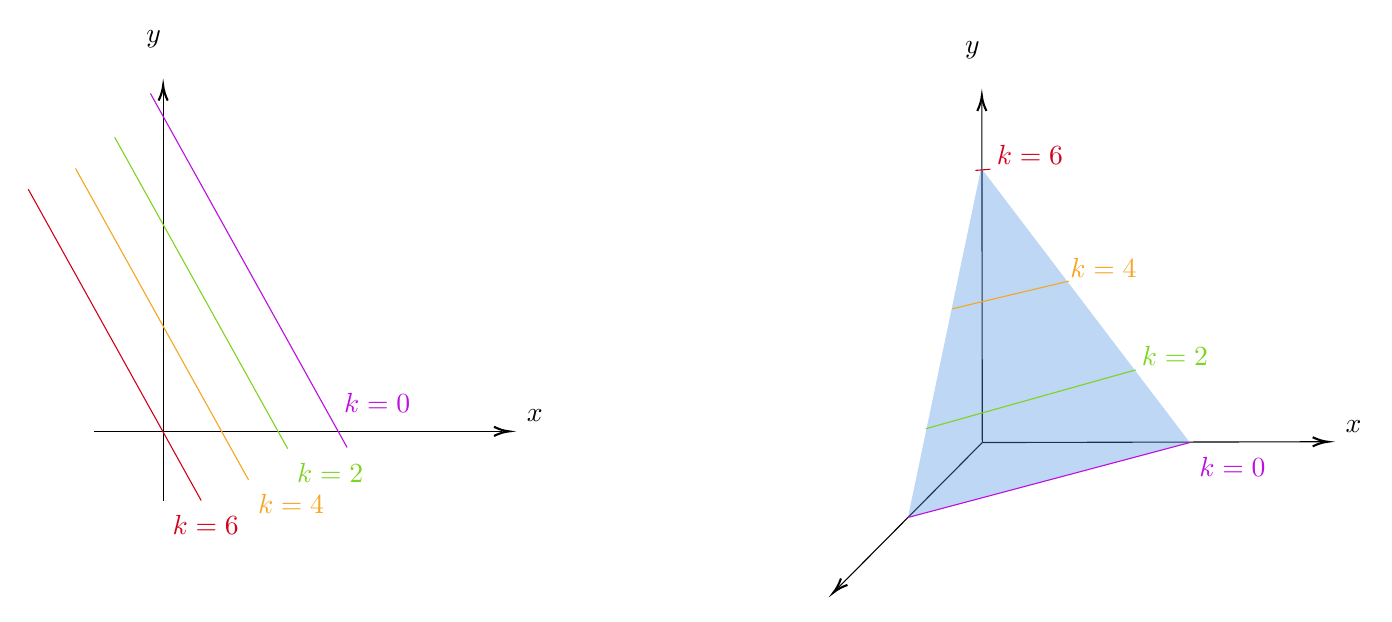
\begin{tikzpicture}[x=1.25pt,y=1.25pt,yscale=-1,xscale=1]
    %uncomment if require: \path (0,300); %set diagram left start at 0, and has height of 300
                    %Straight Lines [id:da8990723361816482] 
                    \draw    (192,208.67) -- (192,90.67) ;
                    \draw [shift={(192,88.67)}, rotate = 90] [color={rgb, 255:red, 0; green, 0; blue, 0 }  ][line width=0.75]    (4.37,-1.32) .. controls (2.78,-0.56) and (1.32,-0.12) .. (0,0) .. controls (1.32,0.12) and (2.78,0.56) .. (4.37,1.32)   ;
                    %Straight Lines [id:da7478280448104192] 
                    \draw    (172,188.67) -- (290,188.67) ;
                    \draw [shift={(292,188.67)}, rotate = 180] [color={rgb, 255:red, 0; green, 0; blue, 0 }  ][line width=0.75]    (4.37,-1.32) .. controls (2.78,-0.56) and (1.32,-0.12) .. (0,0) .. controls (1.32,0.12) and (2.78,0.56) .. (4.37,1.32)   ;
                    %Straight Lines [id:da28676267425737956] 
                    \draw [color={rgb, 255:red, 208; green, 2; blue, 27 }  ,draw opacity=1 ]   (153,118.67) -- (203,208.67) ;
                    %Straight Lines [id:da7277707905157709] 
                    \draw [color={rgb, 255:red, 245; green, 166; blue, 35 }  ,draw opacity=1 ]   (166.67,112.67) -- (216.67,202.67) ;
                    %Straight Lines [id:da7275591847875857] 
                    \draw [color={rgb, 255:red, 126; green, 211; blue, 33 }  ,draw opacity=1 ]   (178,103.67) -- (228,193.67) ;
                    %Straight Lines [id:da8404566915602824] 
                    \draw [color={rgb, 255:red, 189; green, 16; blue, 224 }  ,draw opacity=1 ]   (188.33,91) -- (245.18,193.32) ;
                    %Straight Lines [id:da20264971918684138] 
                    \draw    (428.8,191.9) -- (428.67,93.67) ;
                    \draw [shift={(428.67,91.67)}, rotate = 89.92] [color={rgb, 255:red, 0; green, 0; blue, 0 }  ][line width=0.75]    (4.37,-1.32) .. controls (2.78,-0.56) and (1.32,-0.12) .. (0,0) .. controls (1.32,0.12) and (2.78,0.56) .. (4.37,1.32)   ;
                    %Straight Lines [id:da3198102385142041] 
                    \draw    (428.8,191.9) -- (526.67,191.67) ;
                    \draw [shift={(528.67,191.67)}, rotate = 179.87] [color={rgb, 255:red, 0; green, 0; blue, 0 }  ][line width=0.75]    (4.37,-1.32) .. controls (2.78,-0.56) and (1.32,-0.12) .. (0,0) .. controls (1.32,0.12) and (2.78,0.56) .. (4.37,1.32)   ;
                    %Straight Lines [id:da9181883297393563] 
                    \draw    (428.8,191.9) -- (387.21,233.81) ;
                    \draw [shift={(385.8,235.23)}, rotate = 314.78] [color={rgb, 255:red, 0; green, 0; blue, 0 }  ][line width=0.75]    (4.37,-1.32) .. controls (2.78,-0.56) and (1.32,-0.12) .. (0,0) .. controls (1.32,0.12) and (2.78,0.56) .. (4.37,1.32)   ;
                    %Straight Lines [id:da5374149032464713] 
                    \draw [draw opacity=0][fill={rgb, 255:red, 74; green, 144; blue, 226 }  ,fill opacity=0.36 ]   (428.47,112.57) -- (407.3,213.57) -- (488.8,191.9) -- cycle ;
                    %Straight Lines [id:da6924013277673103] 
                    \draw [color={rgb, 255:red, 189; green, 16; blue, 224 }  ,draw opacity=1 ]   (407.3,213.57) -- (488.8,191.9) ;
                    %Straight Lines [id:da8716167998681623] 
                    \draw [color={rgb, 255:red, 126; green, 211; blue, 33 }  ,draw opacity=1 ]   (412.47,187.9) -- (473.13,170.9) ;
                    %Straight Lines [id:da7369820628309036] 
                    \draw [color={rgb, 255:red, 245; green, 166; blue, 35 }  ,draw opacity=1 ]   (420.13,153.23) -- (453.8,145.23) ;
                    %Straight Lines [id:da7423607072321098] 
                    \draw [color={rgb, 255:red, 208; green, 2; blue, 27 }  ,draw opacity=1 ]   (426.8,113.23) -- (431.13,112.9) ;

                    % Text Node
                    \draw (296.4,181.67) node [anchor=north west][inner sep=0.75pt]  [font=\normalsize]  {$x$};
                    % Text Node
                    \draw (186.4,72.13) node [anchor=north west][inner sep=0.75pt]  [font=\normalsize]  {$y$};
                    % Text Node
                    \draw (194,212.07) node [anchor=north west][inner sep=0.75pt]  [font=\normalsize]  {$\textcolor[rgb]{0.82,0.01,0.11}{k=6}$};
                    % Text Node
                    \draw (218.67,206.07) node [anchor=north west][inner sep=0.75pt]  [font=\normalsize,color={rgb, 255:red, 245; green, 166; blue, 35 }  ,opacity=1 ]  {$\textcolor[rgb]{0.96,0.65,0.14}{k=4}$};
                    % Text Node
                    \draw (230,197.07) node [anchor=north west][inner sep=0.75pt]  [font=\normalsize,color={rgb, 255:red, 245; green, 166; blue, 35 }  ,opacity=1 ]  {$\textcolor[rgb]{0.49,0.83,0.13}{k=2}$};
                    % Text Node
                    \draw (243.56,176.88) node [anchor=north west][inner sep=0.75pt]  [font=\normalsize,color={rgb, 255:red, 245; green, 166; blue, 35 }  ,opacity=1 ]  {$\textcolor[rgb]{0.74,0.06,0.88}{k=0}$};
                    % Text Node
                    \draw (533.07,184.67) node [anchor=north west][inner sep=0.75pt]  [font=\normalsize]  {$x$};
                    % Text Node
                    \draw (423.07,75.13) node [anchor=north west][inner sep=0.75pt]  [font=\normalsize]  {$y$};
                    % Text Node
                    \draw (490.8,195.3) node [anchor=north west][inner sep=0.75pt]  [font=\normalsize,color={rgb, 255:red, 245; green, 166; blue, 35 }  ,opacity=1 ]  {$\textcolor[rgb]{0.74,0.06,0.88}{k=0}$};
                    % Text Node
                    \draw (474.17,163.3) node [anchor=north west][inner sep=0.75pt]  [font=\normalsize,color={rgb, 255:red, 245; green, 166; blue, 35 }  ,opacity=1 ]  {$\textcolor[rgb]{0.49,0.83,0.13}{k=2}$};
                    % Text Node
                    \draw (453.51,137.97) node [anchor=north west][inner sep=0.75pt]  [font=\normalsize,color={rgb, 255:red, 245; green, 166; blue, 35 }  ,opacity=1 ]  {$\textcolor[rgb]{0.96,0.65,0.14}{k=4}$};
                    % Text Node
                    \draw (432.27,105.3) node [anchor=north west][inner sep=0.75pt]  [font=\normalsize,color={rgb, 255:red, 245; green, 166; blue, 35 }  ,opacity=1 ]  {$\textcolor[rgb]{0.82,0.01,0.11}{k=6}$};
                \end{tikzpicture}
            \caption{Curvas de nível e gráfico da função \(f(x,y) = 6 - 3x - 2y\).}
            \label{fig:curvasdenivel1}
        \end{figure}
\end{example}

\begin{example}
    Esboce o gráfico e as curvas de nível da função \(g(x,y) = \sqrt{9 - x^2 - y^2}\) para \(k=0,1,2\) e \(3\).

    Sabemos que \(D_f = \{(x,y)\in\R^2 : x^2 + y^2 \leq 9\}\) e \(\operatorname{Im}_f = [0,3]\), portanto as curvas de nível está bem definidas para \(k\in[0,3]\).
    \begin{itemize}
            \item \(k = 0\): \(g(x,y) = 0 \Rightarrow \sqrt{9 - x^2 - y^2} = 0 \Rightarrow x^2 + y^2 = 9\)
            \item \(k = 1\): \(g(x,y) = 1 \Rightarrow \sqrt{9 - x^2 - y^2} = 1 \Rightarrow x^2 + y^2 = 8\)
            \item \(k = 2\): \(g(x,y) = 0 \Rightarrow \sqrt{9 - x^2 - y^2} = 2 \Rightarrow x^2 + y^2 = 5\)
            \item \(k = 3\): \(g(x,y) = 0 \Rightarrow \sqrt{9 - x^2 - y^2} = 3 \Rightarrow x^2 + y^2 = 0\)
        \end{itemize}
        \begin{figure}[htbp]
            \centering
                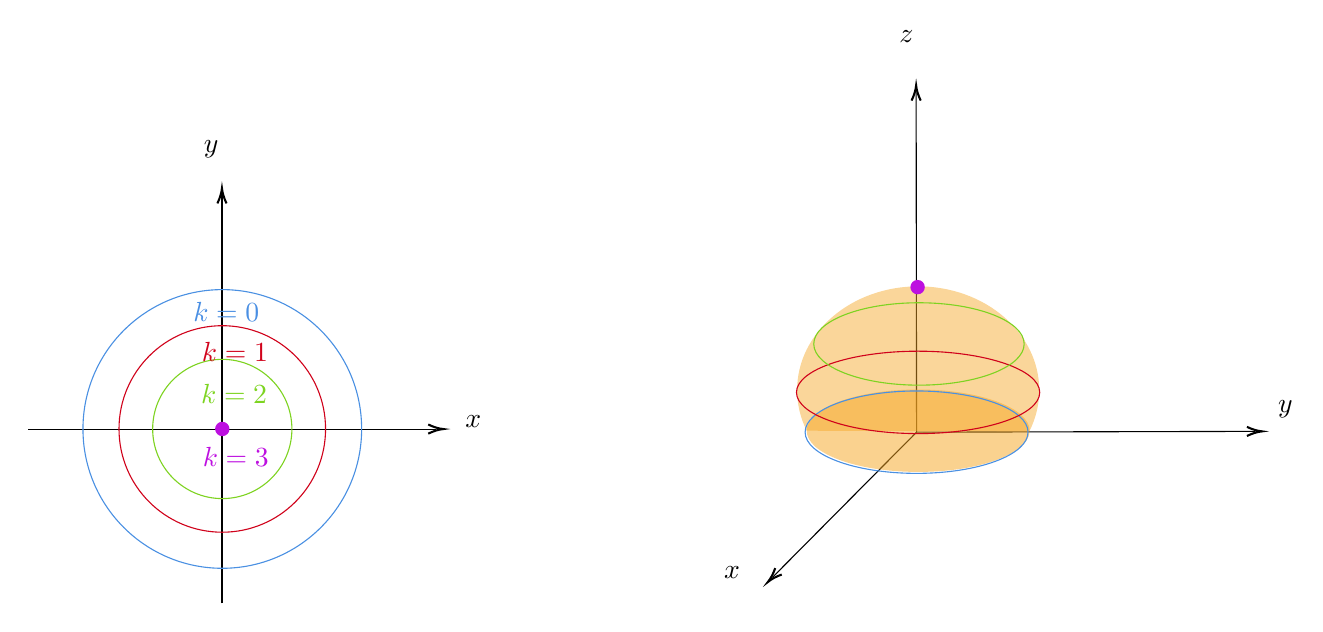
\begin{tikzpicture}[x=1.25pt,y=1.25pt,yscale=-1,xscale=1]
    %uncomment if require: \path (0,300); %set diagram left start at 0, and has height of 300
                    %Straight Lines [id:da9005421899192951] 
                    \draw    (200,229.8) -- (200,111.8) ;
                    \draw [shift={(200,109.8)}, rotate = 90] [color={rgb, 255:red, 0; green, 0; blue, 0 }  ][line width=0.75]    (4.37,-1.32) .. controls (2.78,-0.56) and (1.32,-0.12) .. (0,0) .. controls (1.32,0.12) and (2.78,0.56) .. (4.37,1.32)   ;
                    %Straight Lines [id:da22363777483293845] 
                    \draw    (144,179.4) -- (262,179.4) ;
                    \draw [shift={(264,179.4)}, rotate = 180] [color={rgb, 255:red, 0; green, 0; blue, 0 }  ][line width=0.75]    (4.37,-1.32) .. controls (2.78,-0.56) and (1.32,-0.12) .. (0,0) .. controls (1.32,0.12) and (2.78,0.56) .. (4.37,1.32)   ;
                    %Straight Lines [id:da08360455299313296] 
                    \draw    (400.8,180.3) -- (400.67,82.07) ;
                    \draw [shift={(400.67,80.07)}, rotate = 89.92] [color={rgb, 255:red, 0; green, 0; blue, 0 }  ][line width=0.75]    (4.37,-1.32) .. controls (2.78,-0.56) and (1.32,-0.12) .. (0,0) .. controls (1.32,0.12) and (2.78,0.56) .. (4.37,1.32)   ;
                    %Straight Lines [id:da1255686424003376] 
                    \draw    (400.8,180.3) -- (498.67,180.07) ;
                    \draw [shift={(500.67,180.07)}, rotate = 179.87] [color={rgb, 255:red, 0; green, 0; blue, 0 }  ][line width=0.75]    (4.37,-1.32) .. controls (2.78,-0.56) and (1.32,-0.12) .. (0,0) .. controls (1.32,0.12) and (2.78,0.56) .. (4.37,1.32)   ;
                    %Straight Lines [id:da9713829965193167] 
                    \draw    (400.8,180.3) -- (359.21,222.21) ;
                    \draw [shift={(357.8,223.63)}, rotate = 314.78] [color={rgb, 255:red, 0; green, 0; blue, 0 }  ][line width=0.75]    (4.37,-1.32) .. controls (2.78,-0.56) and (1.32,-0.12) .. (0,0) .. controls (1.32,0.12) and (2.78,0.56) .. (4.37,1.32)   ;
                    %Shape: Circle [id:dp6116890534445036] 
                    \draw  [draw opacity=0][fill={rgb, 255:red, 189; green, 16; blue, 224 }  ,fill opacity=1 ] (198.02,179.37) .. controls (198.02,178.22) and (198.95,177.29) .. (200.1,177.29) .. controls (201.25,177.29) and (202.18,178.22) .. (202.18,179.37) .. controls (202.18,180.52) and (201.25,181.45) .. (200.1,181.45) .. controls (198.95,181.45) and (198.02,180.52) .. (198.02,179.37) -- cycle ;
                    %Shape: Circle [id:dp019052448495683993] 
                    \draw  [color={rgb, 255:red, 126; green, 211; blue, 33 }  ,draw opacity=1 ] (179.97,179.37) .. controls (179.97,168.26) and (188.99,159.25) .. (200.1,159.25) .. controls (211.21,159.25) and (220.22,168.26) .. (220.22,179.37) .. controls (220.22,190.48) and (211.21,199.5) .. (200.1,199.5) .. controls (188.99,199.5) and (179.97,190.48) .. (179.97,179.37) -- cycle ;
                    %Shape: Circle [id:dp517180935046544] 
                    \draw  [color={rgb, 255:red, 208; green, 2; blue, 27 }  ,draw opacity=1 ] (170.24,179.37) .. controls (170.24,162.88) and (183.61,149.52) .. (200.1,149.52) .. controls (216.59,149.52) and (229.95,162.88) .. (229.95,179.37) .. controls (229.95,195.86) and (216.59,209.22) .. (200.1,209.22) .. controls (183.61,209.22) and (170.24,195.86) .. (170.24,179.37) -- cycle ;
                    %Shape: Circle [id:dp6339164611040847] 
                    \draw  [color={rgb, 255:red, 74; green, 144; blue, 226 }  ,draw opacity=1 ] (159.82,179.37) .. controls (159.82,157.12) and (177.85,139.09) .. (200.1,139.09) .. controls (222.35,139.09) and (240.38,157.12) .. (240.38,179.37) .. controls (240.38,201.62) and (222.35,219.65) .. (200.1,219.65) .. controls (177.85,219.65) and (159.82,201.62) .. (159.82,179.37) -- cycle ;
                    %Flowchart: Connector [id:dp6414617703668187] 
                    \draw  [draw opacity=0][fill={rgb, 255:red, 245; green, 166; blue, 35 }  ,fill opacity=0.51 ] (369.04,179.88) .. controls (369.04,173.3) and (383.47,167.97) .. (401.26,167.97) .. controls (419.06,167.97) and (433.49,173.3) .. (433.49,179.88) .. controls (433.49,186.45) and (419.06,191.79) .. (401.26,191.79) .. controls (383.47,191.79) and (369.04,186.45) .. (369.04,179.88) -- cycle ;
                    %Shape: Chord [id:dp6504135876557121] 
                    \draw  [draw opacity=0][fill={rgb, 255:red, 245; green, 166; blue, 35 }  ,fill opacity=0.46 ] (369.04,179.88) .. controls (367.25,176.27) and (366.26,172.31) .. (366.26,168.15) .. controls (366.26,151.58) and (381.93,138.15) .. (401.26,138.15) .. controls (420.59,138.15) and (436.26,151.58) .. (436.26,168.15) .. controls (436.26,172.38) and (435.24,176.41) .. (433.4,180.06) -- cycle ;
                    %Flowchart: Connector [id:dp925863392347943] 
                    \draw  [color={rgb, 255:red, 74; green, 144; blue, 226 }  ,draw opacity=1 ] (368.58,180.3) .. controls (368.58,173.72) and (383,168.39) .. (400.8,168.39) .. controls (418.6,168.39) and (433.02,173.72) .. (433.02,180.3) .. controls (433.02,186.88) and (418.6,192.21) .. (400.8,192.21) .. controls (383,192.21) and (368.58,186.88) .. (368.58,180.3) -- cycle ;
                    %Flowchart: Connector [id:dp05038336129863108] 
                    \draw  [color={rgb, 255:red, 208; green, 2; blue, 27 }  ,draw opacity=1 ] (366.08,168.8) .. controls (366.08,162.22) and (381.82,156.89) .. (401.24,156.89) .. controls (420.66,156.89) and (436.4,162.22) .. (436.4,168.8) .. controls (436.4,175.38) and (420.66,180.71) .. (401.24,180.71) .. controls (381.82,180.71) and (366.08,175.38) .. (366.08,168.8) -- cycle ;
                    %Flowchart: Connector [id:dp616582824034949] 
                    \draw  [color={rgb, 255:red, 126; green, 211; blue, 33 }  ,draw opacity=1 ] (371.08,154.8) .. controls (371.08,148.22) and (384.69,142.89) .. (401.49,142.89) .. controls (418.28,142.89) and (431.9,148.22) .. (431.9,154.8) .. controls (431.9,161.38) and (418.28,166.71) .. (401.49,166.71) .. controls (384.69,166.71) and (371.08,161.38) .. (371.08,154.8) -- cycle ;
                    %Shape: Circle [id:dp8982011313141853] 
                    \draw  [draw opacity=0][fill={rgb, 255:red, 189; green, 16; blue, 224 }  ,fill opacity=1 ] (399.02,138.37) .. controls (399.02,137.22) and (399.95,136.29) .. (401.1,136.29) .. controls (402.25,136.29) and (403.18,137.22) .. (403.18,138.37) .. controls (403.18,139.52) and (402.25,140.45) .. (401.1,140.45) .. controls (399.95,140.45) and (399.02,139.52) .. (399.02,138.37) -- cycle ;

                    % Text Node
                    \draw (269.6,174.8) node [anchor=north west][inner sep=0.75pt]  [font=\normalsize]  {$x$};
                    % Text Node
                    \draw (194,95.27) node [anchor=north west][inner sep=0.75pt]  [font=\normalsize]  {$y$};
                    % Text Node
                    \draw (344.4,218.4) node [anchor=north west][inner sep=0.75pt]  [font=\normalsize]  {$x$};
                    % Text Node
                    \draw (395.07,63.53) node [anchor=north west][inner sep=0.75pt]  [font=\normalsize]  {$z$};
                    % Text Node
                    \draw (193.7,183.85) node [anchor=north west][inner sep=0.75pt]  [font=\normalsize]  {$\textcolor[rgb]{0.74,0.06,0.88}{k=3}$};
                    % Text Node
                    \draw (193.2,165.8) node [anchor=north west][inner sep=0.75pt]  [font=\normalsize]  {$\textcolor[rgb]{0.49,0.83,0.13}{k=2}$};
                    % Text Node
                    \draw (193.45,153.5) node [anchor=north west][inner sep=0.75pt]  [font=\normalsize]  {$\textcolor[rgb]{0.82,0.01,0.11}{k=1}$};
                    % Text Node
                    \draw (190.95,142) node [anchor=north west][inner sep=0.75pt]  [font=\normalsize]  {$\textcolor[rgb]{0.29,0.56,0.89}{k=0}$};
                    % Text Node
                    \draw (504.53,170.53) node [anchor=north west][inner sep=0.75pt]    {$y$};

                \end{tikzpicture}
            \caption{Curvas de nível e gráfico da função \(f(x,y) = \sqrt{9-x^2-y^2}\).}
            \label{fig:curvasdenivel2}
        \end{figure}
\end{example}

\begin{example}
    Seja \(f(x,y) = \frac{1}{x^2 + y^2}\). Determine o domínio e a imagem de \(f\). Em seguida esboce suas curvas de nível e gráfico.

    É claro que \(D_f = \{(x,y)\in\R^2 : (x,y)\neq (0,0)\}\) e \[\operatorname{Im}_f = \{z=f(x,y) : (x,y)\in D_f\} = \left\{ x = \frac{1}{x^2 + y^2} : (x,y)\neq(0,0) \right\} = (0,\infty).\] Além disso, para \(k>0\) temos \[\frac{1}{x^2 + y^2} = k \Rightarrow x^2 + y^2 = \frac{1}{k},\] portanto as curvas de nível são circunferências concêntricas de raio \(\sqrt{\frac{1}{k}}\). Observe que quando \(k\) é pequeno, o raio da circunferência é grande, e quando \(k\) é grande, o raio é pequeno. Além disso, note que, se \(x=0\), então \(z = \frac{1}{y^2}\) é uma hiperbole no plano yz; agora se \(y=0\), \(z = \frac{1}{x^2}\) é uma hiperbole no plano xz. Com essas informações podemos esboçar as curvas de nível e o gráfico de \(f\).
\begin{figure}[htbp]
            \centering
                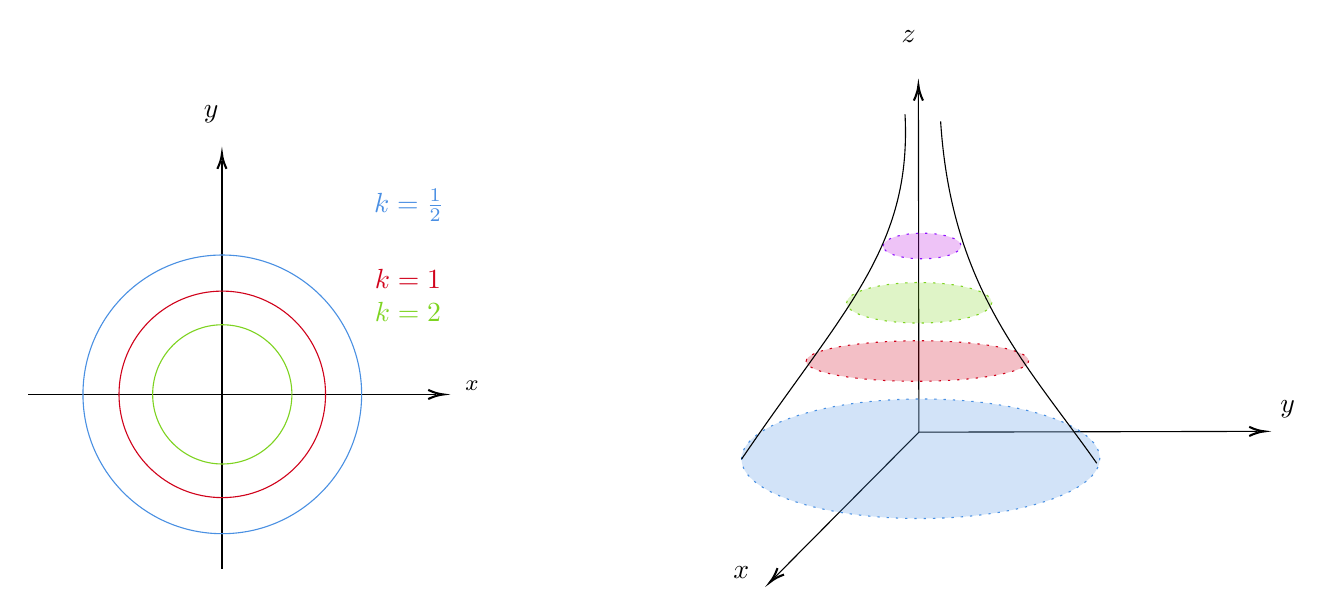
\begin{tikzpicture}[x=1.25pt,y=1.25pt,yscale=-1,xscale=1]
    %uncomment if require: \path (0,300); %set diagram left start at 0, and has height of 300
                    %Straight Lines [id:da24437428975701714] 
                    \draw    (80.67,206.8) -- (80.67,88.8) ;
                    \draw [shift={(80.67,86.8)}, rotate = 90] [color={rgb, 255:red, 0; green, 0; blue, 0 }  ][line width=0.75]    (4.37,-1.32) .. controls (2.78,-0.56) and (1.32,-0.12) .. (0,0) .. controls (1.32,0.12) and (2.78,0.56) .. (4.37,1.32)   ;
                    %Straight Lines [id:da10202597957111392] 
                    \draw    (24.67,156.4) -- (142.67,156.4) ;
                    \draw [shift={(144.67,156.4)}, rotate = 180] [color={rgb, 255:red, 0; green, 0; blue, 0 }  ][line width=0.75]    (4.37,-1.32) .. controls (2.78,-0.56) and (1.32,-0.12) .. (0,0) .. controls (1.32,0.12) and (2.78,0.56) .. (4.37,1.32)   ;
                    %Straight Lines [id:da03442276412344114] 
                    \draw    (282.13,167.3) -- (282,69.07) ;
                    \draw [shift={(282,67.07)}, rotate = 89.92] [color={rgb, 255:red, 0; green, 0; blue, 0 }  ][line width=0.75]    (4.37,-1.32) .. controls (2.78,-0.56) and (1.32,-0.12) .. (0,0) .. controls (1.32,0.12) and (2.78,0.56) .. (4.37,1.32)   ;
                    %Straight Lines [id:da8565157872425141] 
                    \draw    (282.13,167.3) -- (380,167.07) ;
                    \draw [shift={(382,167.07)}, rotate = 179.87] [color={rgb, 255:red, 0; green, 0; blue, 0 }  ][line width=0.75]    (4.37,-1.32) .. controls (2.78,-0.56) and (1.32,-0.12) .. (0,0) .. controls (1.32,0.12) and (2.78,0.56) .. (4.37,1.32)   ;
                    %Straight Lines [id:da005485083537555058] 
                    \draw    (282.13,167.3) -- (240.54,209.21) ;
                    \draw [shift={(239.13,210.63)}, rotate = 314.78] [color={rgb, 255:red, 0; green, 0; blue, 0 }  ][line width=0.75]    (4.37,-1.32) .. controls (2.78,-0.56) and (1.32,-0.12) .. (0,0) .. controls (1.32,0.12) and (2.78,0.56) .. (4.37,1.32)   ;
                    %Shape: Circle [id:dp8256132701254346] 
                    \draw  [color={rgb, 255:red, 126; green, 211; blue, 33 }  ,draw opacity=1 ] (60.64,156.37) .. controls (60.64,145.26) and (69.65,136.25) .. (80.77,136.25) .. controls (91.88,136.25) and (100.89,145.26) .. (100.89,156.37) .. controls (100.89,167.48) and (91.88,176.5) .. (80.77,176.5) .. controls (69.65,176.5) and (60.64,167.48) .. (60.64,156.37) -- cycle ;
                    %Shape: Circle [id:dp1765127823583098] 
                    \draw  [color={rgb, 255:red, 208; green, 2; blue, 27 }  ,draw opacity=1 ] (50.91,156.37) .. controls (50.91,139.88) and (64.28,126.52) .. (80.77,126.52) .. controls (97.26,126.52) and (110.62,139.88) .. (110.62,156.37) .. controls (110.62,172.86) and (97.26,186.22) .. (80.77,186.22) .. controls (64.28,186.22) and (50.91,172.86) .. (50.91,156.37) -- cycle ;
                    %Shape: Circle [id:dp6534693648452948] 
                    \draw  [color={rgb, 255:red, 74; green, 144; blue, 226 }  ,draw opacity=1 ] (40.49,156.37) .. controls (40.49,134.12) and (58.52,116.09) .. (80.77,116.09) .. controls (103.01,116.09) and (121.05,134.12) .. (121.05,156.37) .. controls (121.05,178.62) and (103.01,196.65) .. (80.77,196.65) .. controls (58.52,196.65) and (40.49,178.62) .. (40.49,156.37) -- cycle ;
                    %Flowchart: Connector [id:dp20357625150336012] 
                    \draw  [color={rgb, 255:red, 208; green, 2; blue, 27 }  ,draw opacity=1 ][fill={rgb, 255:red, 208; green, 2; blue, 27 }  ,fill opacity=0.25 ][dash pattern={on 0.84pt off 2.51pt}] (249.56,146.81) .. controls (249.55,143.58) and (263.93,140.92) .. (281.69,140.88) .. controls (299.44,140.83) and (313.84,143.42) .. (313.85,146.66) .. controls (313.86,149.89) and (299.47,152.55) .. (281.72,152.59) .. controls (263.96,152.64) and (249.57,150.05) .. (249.56,146.81) -- cycle ;
                    %Flowchart: Connector [id:dp728442972792305] 
                    \draw  [color={rgb, 255:red, 74; green, 144; blue, 226 }  ,draw opacity=1 ][fill={rgb, 255:red, 74; green, 144; blue, 226 }  ,fill opacity=0.25 ][dash pattern={on 0.84pt off 2.51pt}] (230.88,175.11) .. controls (230.85,165.57) and (254.01,157.78) .. (282.61,157.71) .. controls (311.2,157.64) and (334.4,165.31) .. (334.42,174.86) .. controls (334.45,184.4) and (311.29,192.19) .. (282.69,192.26) .. controls (254.1,192.33) and (230.9,184.65) .. (230.88,175.11) -- cycle ;
                    %Flowchart: Connector [id:dp8540526439832161] 
                    \draw  [color={rgb, 255:red, 126; green, 211; blue, 33 }  ,draw opacity=1 ][fill={rgb, 255:red, 126; green, 211; blue, 33 }  ,fill opacity=0.25 ][dash pattern={on 0.84pt off 2.51pt}] (261.22,129.95) .. controls (261.22,126.71) and (270.61,124.07) .. (282.21,124.04) .. controls (293.81,124.01) and (303.22,126.61) .. (303.22,129.85) .. controls (303.23,133.08) and (293.84,135.73) .. (282.24,135.76) .. controls (270.64,135.78) and (261.23,133.18) .. (261.22,129.95) -- cycle ;
                    %Flowchart: Connector [id:dp14611648575471736] 
                    \draw  [color={rgb, 255:red, 144; green, 19; blue, 254 }  ,draw opacity=1 ][fill={rgb, 255:red, 189; green, 16; blue, 224 }  ,fill opacity=0.25 ][dash pattern={on 0.84pt off 2.51pt}] (271.77,113.51) .. controls (271.77,111.47) and (276.81,109.8) .. (283.04,109.78) .. controls (289.27,109.77) and (294.33,111.41) .. (294.34,113.46) .. controls (294.34,115.5) and (289.29,117.17) .. (283.06,117.18) .. controls (276.83,117.2) and (271.78,115.55) .. (271.77,113.51) -- cycle ;
                    %Curve Lines [id:da860309563236923] 
                    \draw    (230.88,175.11) .. controls (260.13,132) and (280.13,114.29) .. (278.13,75.43) ;
                    %Curve Lines [id:da9346030576531226] 
                    \draw    (288.42,77.43) .. controls (291.56,126) and (312.99,147.14) .. (333.56,176.29) ;

                    % Text Node
                    \draw (150.27,151.8) node [anchor=north west][inner sep=0.75pt]  [font=\footnotesize]  {$x$};
                    % Text Node
                    \draw (74.67,72.27) node [anchor=north west][inner sep=0.75pt]  [font=\normalsize]  {$y$};
                    % Text Node
                    \draw (227.73,205.4) node [anchor=north west][inner sep=0.75pt]  [font=\normalsize]  {$x$};
                    % Text Node
                    \draw (276.4,50.53) node [anchor=north west][inner sep=0.75pt]  [font=\normalsize]  {$z$};
                    % Text Node
                    \draw (124.15,129.09) node [anchor=north west][inner sep=0.75pt]  [font=\normalsize]  {$\textcolor[rgb]{0.49,0.83,0.13}{k=2}$};
                    % Text Node
                    \draw (124.12,119.36) node [anchor=north west][inner sep=0.75pt]  [font=\normalsize]  {$\textcolor[rgb]{0.82,0.01,0.11}{k=1}$};
                    % Text Node
                    \draw (123.9,96.14) node [anchor=north west][inner sep=0.75pt]  [font=\normalsize]  {$\textcolor[rgb]{0.29,0.56,0.89}{k=\frac{1}{2}}$};
                    % Text Node
                    \draw (385.87,157.53) node [anchor=north west][inner sep=0.75pt]    {$y$};
                \end{tikzpicture}
            \caption{Curvas de nível e gráfico da função \(f(x,y) = \frac{1}{x^2+y^2}\).}
            \label{fig:curvasdenivel3}
        \end{figure}
\end{example}

\begin{exercise}
    \begin{enumerate}
        \item Desenhe as curvas de nível e esboce o gráfico de \(f(x,y) = x^2 + y^2\).
        \item Seja \(f(x,y) = \frac{y}{x-1}\).
            \begin{enumerate}
                \item Determine \(D_f\) e \(\operatorname{Im}_f\).
                \item Desenhe as curvas de nível para \(k = -1,0,1\) e \(2\).
                \item Tente imaginar e esboçar o gráfico de \(f\).
            \end{enumerate}
    \end{enumerate}
\end{exercise}

\section{Funções de 3 variáveis e superfícies de nível}

\begin{definition}\index{Funções de três variáveis reais a valores reais}
    Uma \textbf{função de três variáveis a valores reais}, definida em \(D_f \subset\R^3\), é uma função que associa a cada terna ordenada \((x,y,z)\in D_f\) a um único número real \(w = f(x,y,z)\).
\end{definition}

\begin{definition}\index{Funções de três variáveis reais a valores reais! Gráfico}
    O \textbf{gráfico} de uma função de 3 variáveis é o conjunto \[G_f = \{(x,y,z,w)\in\R^4 : w = f(x,y,z),\, (x,y,z)\in D_f\}.\]
\end{definition}

% Infelizmente não conseguimos nem ao menos imaginar o gráfico de uma função de três variáveis. Para ganharmos um pouco de intuição acerca de seu comportamento, desenhamos suas superfícies de nível.

\begin{definition}\index{Funções de três variáveis reais a valores reais! Superfícies de nível}
    Sejam \(f:D_f\subset\R^3 \to \R\) uma função e \(k\in\operatorname{Im}_f\). O conjunto dos pontos \((x,y,z)\in D_f\) tais que \(f(x,y,z) = k\) é chamado de superfície de nível \(k\) de \(f\).
\end{definition}

Observe que se um ponto se move ao longo de uma superfície de nível, o valor de \(f(x,y,z)\) permanece fixo.

\begin{example}
    Determine as superfícies de nível de \(f(x,y,z) = x^2 + y^2 + z^2\).

    Temos \(D_f = \R^3\) e \[\operatorname{Im}_f = \{ w = x^2 + y^2 + z^2 : (x,y,z)\in\R^3 \} = \{w\geq\} = [0,\infty).\] Portanto, para \(k\geq 0\) temos \[f(x,y,z) = k \Leftrightarrow x^2 + y^2 + z^2 = k,\] ou seja, as superfícies de nível de \(f\) são esferas concêntricas de raio \(\sqrt{k}\) centradas na origem.
        \begin{figure}[htbp]
            \centering
                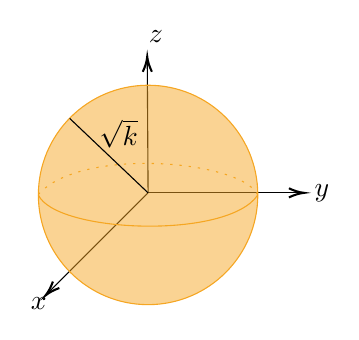
\begin{tikzpicture}[x=0.5pt,y=0.5pt,yscale=-1,xscale=1]
                    %Straight Lines [id:da14017589294902055] 
                    \draw    (310.62,189.37) -- (421.33,189.37) ;
                    \draw [shift={(423.33,189.37)}, rotate = 180] [color={rgb, 255:red, 0; green, 0; blue, 0 }  ][line width=0.75]    (10.93,-3.29) .. controls (6.95,-1.4) and (3.31,-0.3) .. (0,0) .. controls (3.31,0.3) and (6.95,1.4) .. (10.93,3.29)   ;
                    %Straight Lines [id:da5897002846299654] 
                    \draw    (310.62,189.37) -- (237.84,262.15) ;
                    \draw [shift={(236.43,263.56)}, rotate = 315] [color={rgb, 255:red, 0; green, 0; blue, 0 }  ][line width=0.75]    (10.93,-3.29) .. controls (6.95,-1.4) and (3.31,-0.3) .. (0,0) .. controls (3.31,0.3) and (6.95,1.4) .. (10.93,3.29)   ;
                    %Straight Lines [id:da09863498649444669] 
                    \draw    (310.62,189.37) -- (310.01,92.93) ;
                    \draw [shift={(310,90.93)}, rotate = 89.64] [color={rgb, 255:red, 0; green, 0; blue, 0 }  ][line width=0.75]    (10.93,-3.29) .. controls (6.95,-1.4) and (3.31,-0.3) .. (0,0) .. controls (3.31,0.3) and (6.95,1.4) .. (10.93,3.29)   ;
                    %Flowchart: Connector [id:dp362548466234239] 
                    \draw  [color={rgb, 255:red, 245; green, 166; blue, 35 }  ,draw opacity=1 ][fill={rgb, 255:red, 245; green, 166; blue, 35 }  ,fill opacity=0.49 ] (231.33,190.89) .. controls (231.33,147.1) and (266.83,111.6) .. (310.62,111.6) .. controls (354.41,111.6) and (389.9,147.1) .. (389.9,190.89) .. controls (389.9,234.67) and (354.41,270.17) .. (310.62,270.17) .. controls (266.83,270.17) and (231.33,234.67) .. (231.33,190.89) -- cycle ;
                    %Curve Lines [id:da7713828157202779] 
                    \draw [color={rgb, 255:red, 245; green, 166; blue, 35 }  ,draw opacity=1 ]   (231.33,190.89) .. controls (243.78,218.28) and (368.28,223.54) .. (389.9,190.89) ;
                    %Curve Lines [id:da464364501204271] 
                    \draw [color={rgb, 255:red, 245; green, 166; blue, 35 }  ,draw opacity=1 ] [dash pattern={on 0.84pt off 2.51pt}]  (231.33,190.5) .. controls (262.16,155.77) and (377.73,165.75) .. (389.9,190.89) ;

                    %Straight Lines [id:da2558629543380908] 
                    \draw    (254,135.6) -- (310.62,189.37) ;

                    % Text Node
                    \draw (224,263.4) node [anchor=north west][inner sep=0.75pt]    {$x$};
                    % Text Node
                    \draw (429,181.4) node [anchor=north west][inner sep=0.75pt]    {$y$};
                    % Text Node
                    \draw (309.33,70.4) node [anchor=north west][inner sep=0.75pt]    {$z$};
                    % Text Node
                    \draw (273.57,134.43) node [anchor=north west][inner sep=0.75pt]  [font=\normalsize]  {$\sqrt{k}$};
                \end{tikzpicture}
            \caption{Superfícies de nível da função \(f(x,y,z) = x^2+y^2+z^2\).}
            \label{fig:superficiedenivel}
        \end{figure}
\end{example}

\begin{exercise}
    Esboce as superfícies de nível da função \(f(x,y,z) = y\).
\end{exercise}